Once we have decided to use an FPGA for our application or even just decided to try one out, having an idea of how to write code to see good performance is important. This section describes topics that highlight important concepts and covers a few topics that often cause confusion, to make getting started faster.\par

\hspace*{\fill} \par %插入空行
\textbf{Exposing Parallelism}

We have already looked at how pipeline parallelism is used to efficiently perform work on an FPGA. Another simple pipeline example is shown in Figure 17-12.\par

\hspace*{\fill} \par %插入空行
Figure 17-12. Simple pipeline with five stages: Six clock cycles to process an element of data
\begin{center}
	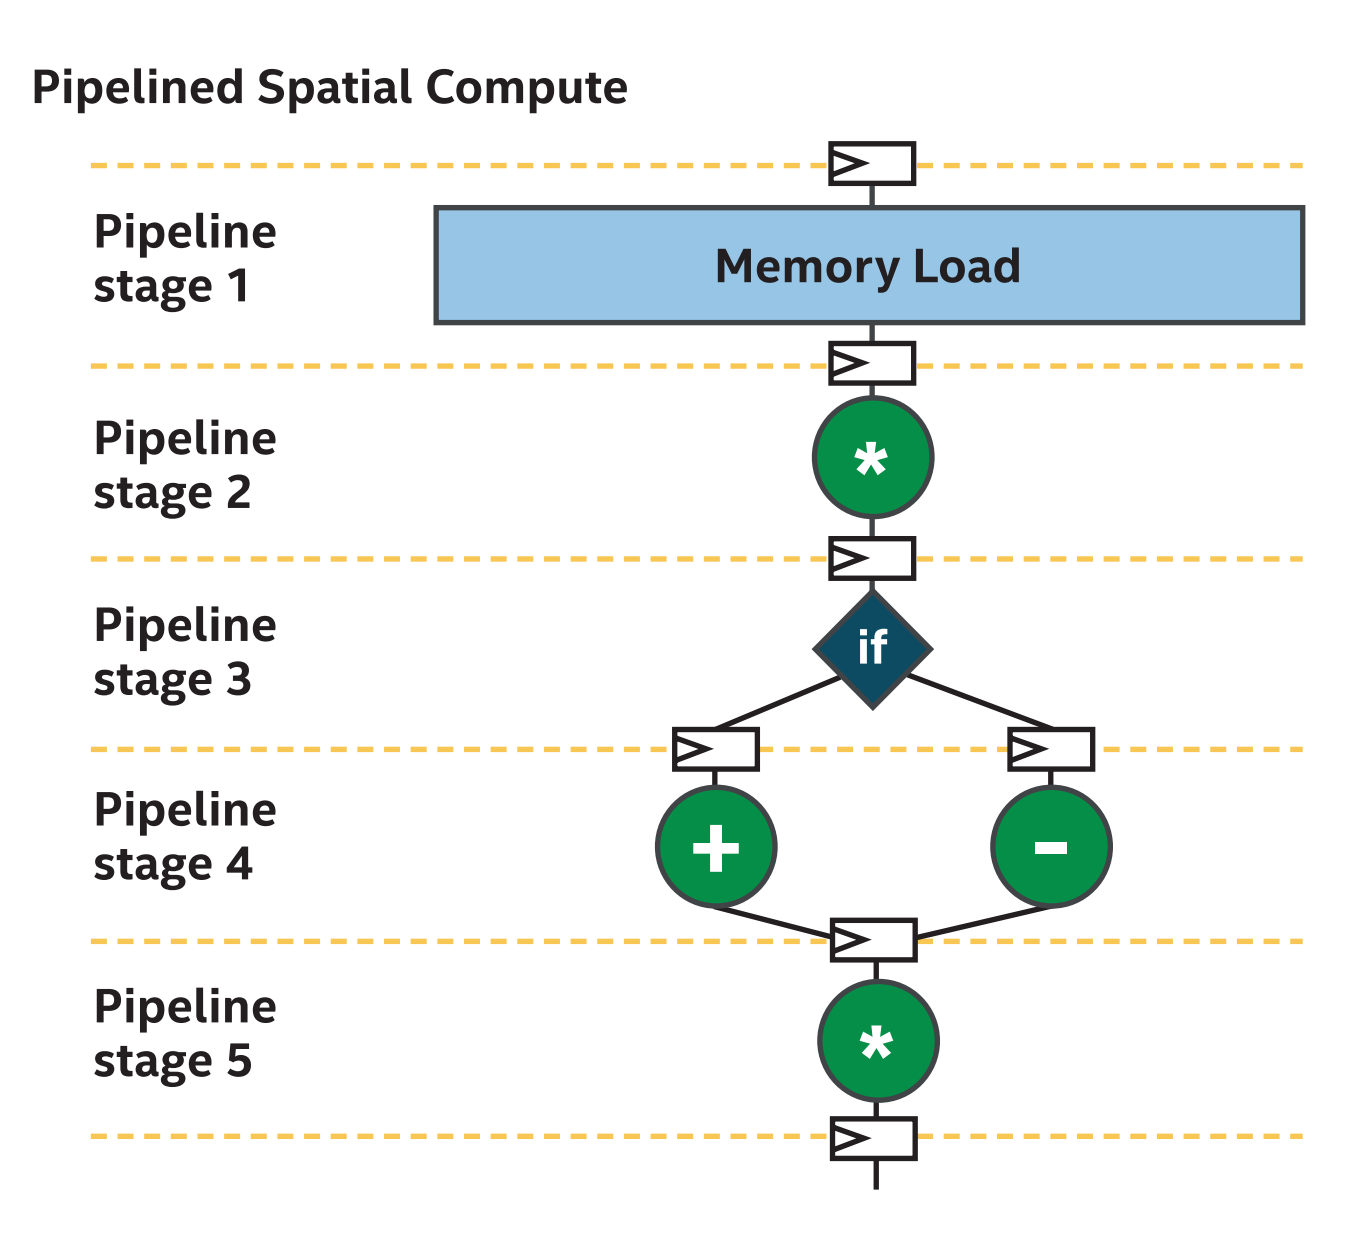
\includegraphics[width=1.0\textwidth]{content/chapter-17/images/11}
\end{center}

In this pipeline, there are five stages. Data moves from one stage to the next once per clock cycle, so in this very simple example, it takes six clock cycles from when data enters into stage 1 until it exits from stage 5.\par

A major goal of pipelining is to enable multiple elements of data to be processed at different stages of the pipeline, simultaneously. To be sure that this is clear, Figure 17-13 shows a pipeline where there is not enough work (only one element of data in this case), which causes each pipeline stage to be unused during most of the clock cycles. This is an inefficient use of the FPGA resources because most of the hardware is idle most of the time.\par

\hspace*{\fill} \par %插入空行
Figure 17-13. Pipeline stages are mostly unused if processing only a single element of work
\begin{center}
	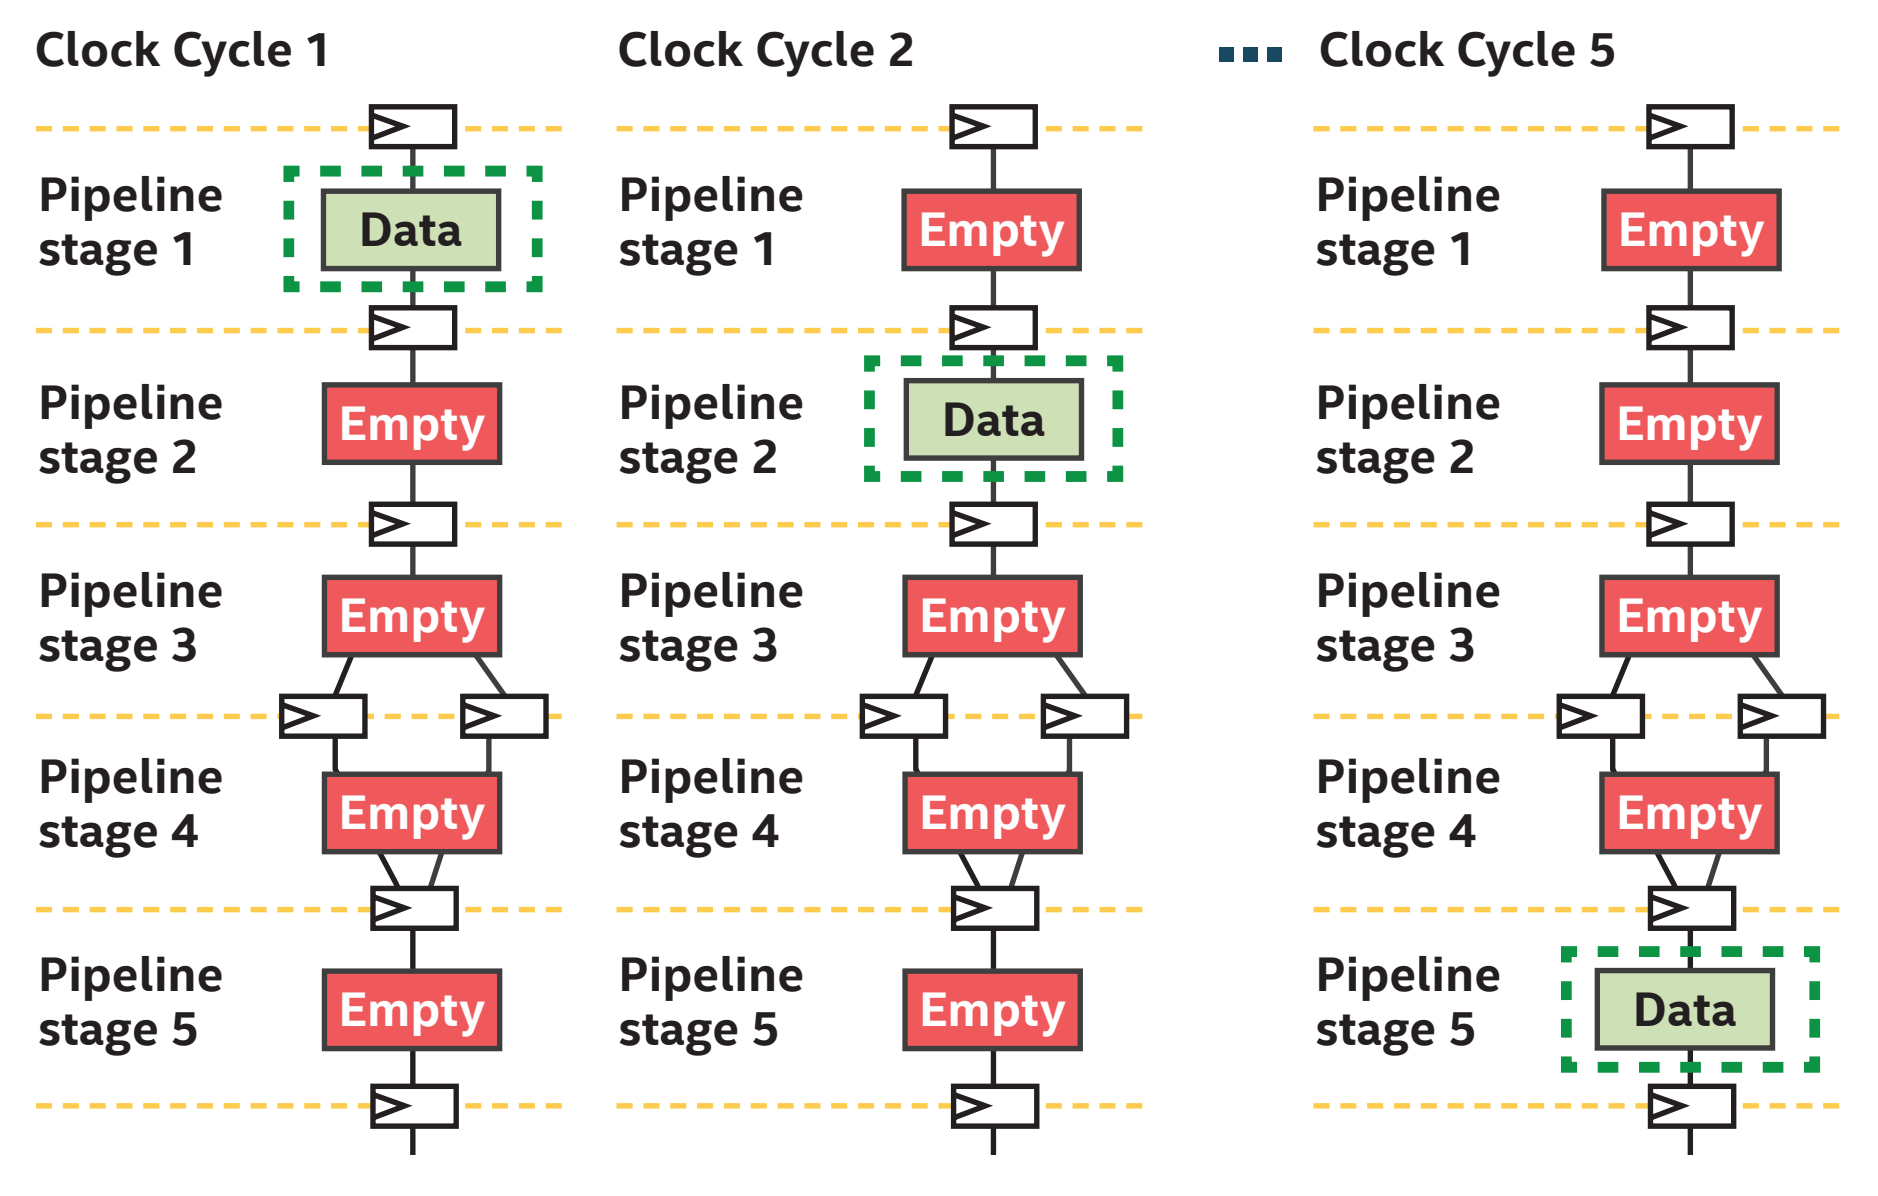
\includegraphics[width=1.0\textwidth]{content/chapter-17/images/12}
\end{center}

To keep the pipeline stages better occupied, it is useful to imagine a queue of un-started work waiting before the first stage, which feeds the pipeline. Each clock cycle, the pipeline can consume and start one more element of work from the queue, as shown in Figure 17-14. After some initial startup cycles, each stage of the pipeline is occupied and doing useful work every clock cycle, leading to efficient utilization of the FPGA resources.\par

\hspace*{\fill} \par %插入空行
Figure 17-14. Efficient utilization comes when each pipeline stage is kept busy
\begin{center}
	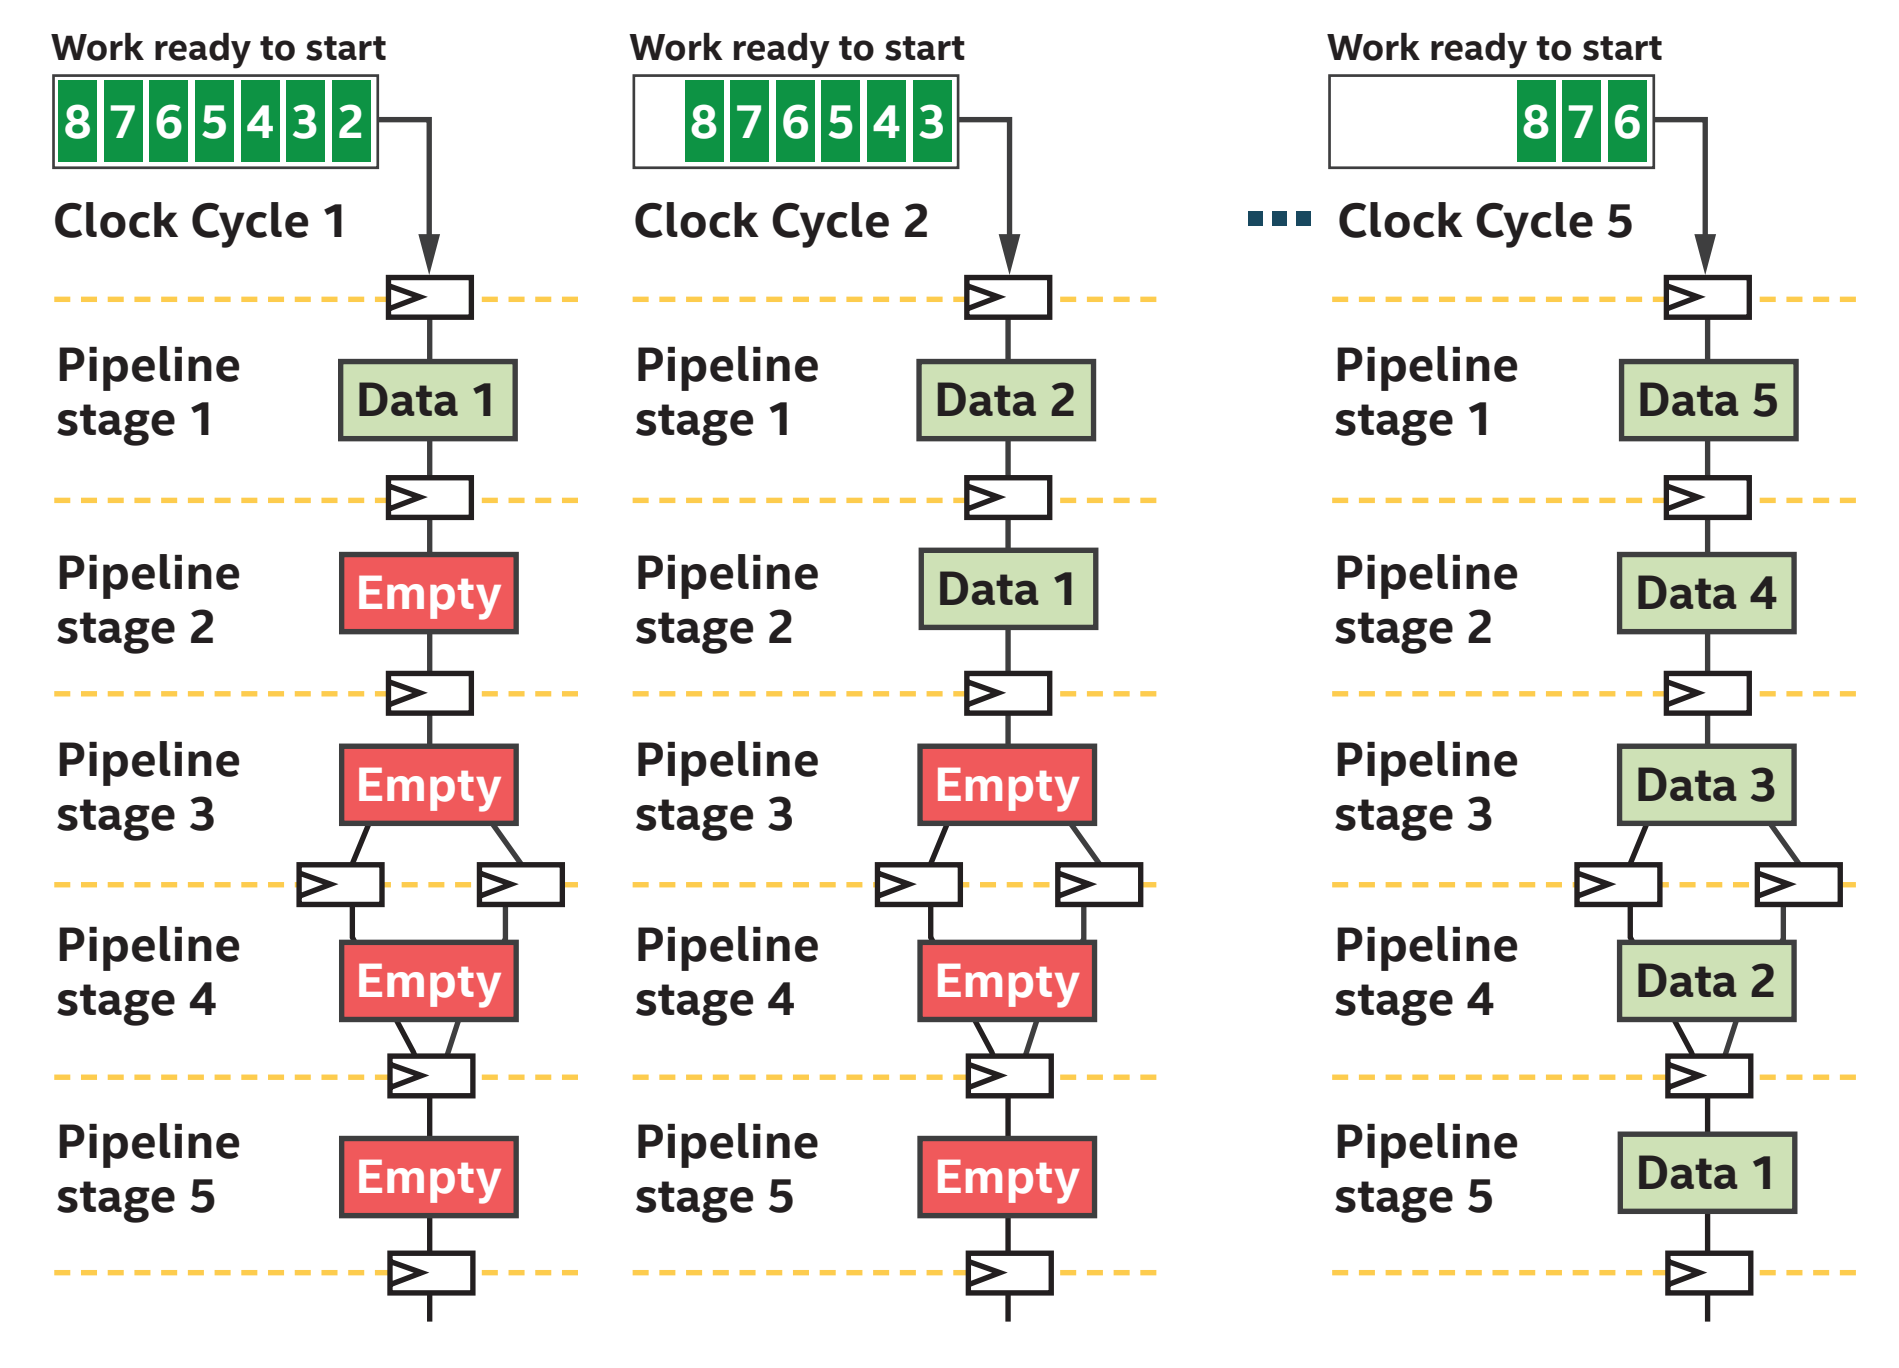
\includegraphics[width=1.0\textwidth]{content/chapter-17/images/13}
\end{center}

The following two sections cover methods to keep the queue feeding the pipeline filled with work that is ready to start. We’ll look at\par

\begin{enumerate}
	\item ND-range kernels
	\item Loops
\end{enumerate}

Choosing between these options impacts how kernels that run on an FPGA should be fundamentally architected. In some cases, algorithms lend themselves well to one style or the other, and in other cases programmer preference and experience inform which method should be chosen.\par

\hspace*{\fill} \par %插入空行
\textbf{Keeping the Pipeline Busy Using ND-Ranges}

The ND-range hierarchical execution model was described in Chapter 4. Figure 17-15 illustrates the key concepts: an ND-range execution model where there is a hierarchical grouping of work-items, and where a workitem is the primitive unit of work that a kernel defines. This model was originally developed to enable efficient programming of GPUs where work-items may execute concurrently at various levels of the execution model hierarchy. To match the type of work that GPU hardware is efficient at, ND-range work-items do not frequently communicate with each other in most applications.\par

\hspace*{\fill} \par %插入空行
Figure 17-15. ND-range execution model: A hierarchical grouping of work-items
\begin{center}
	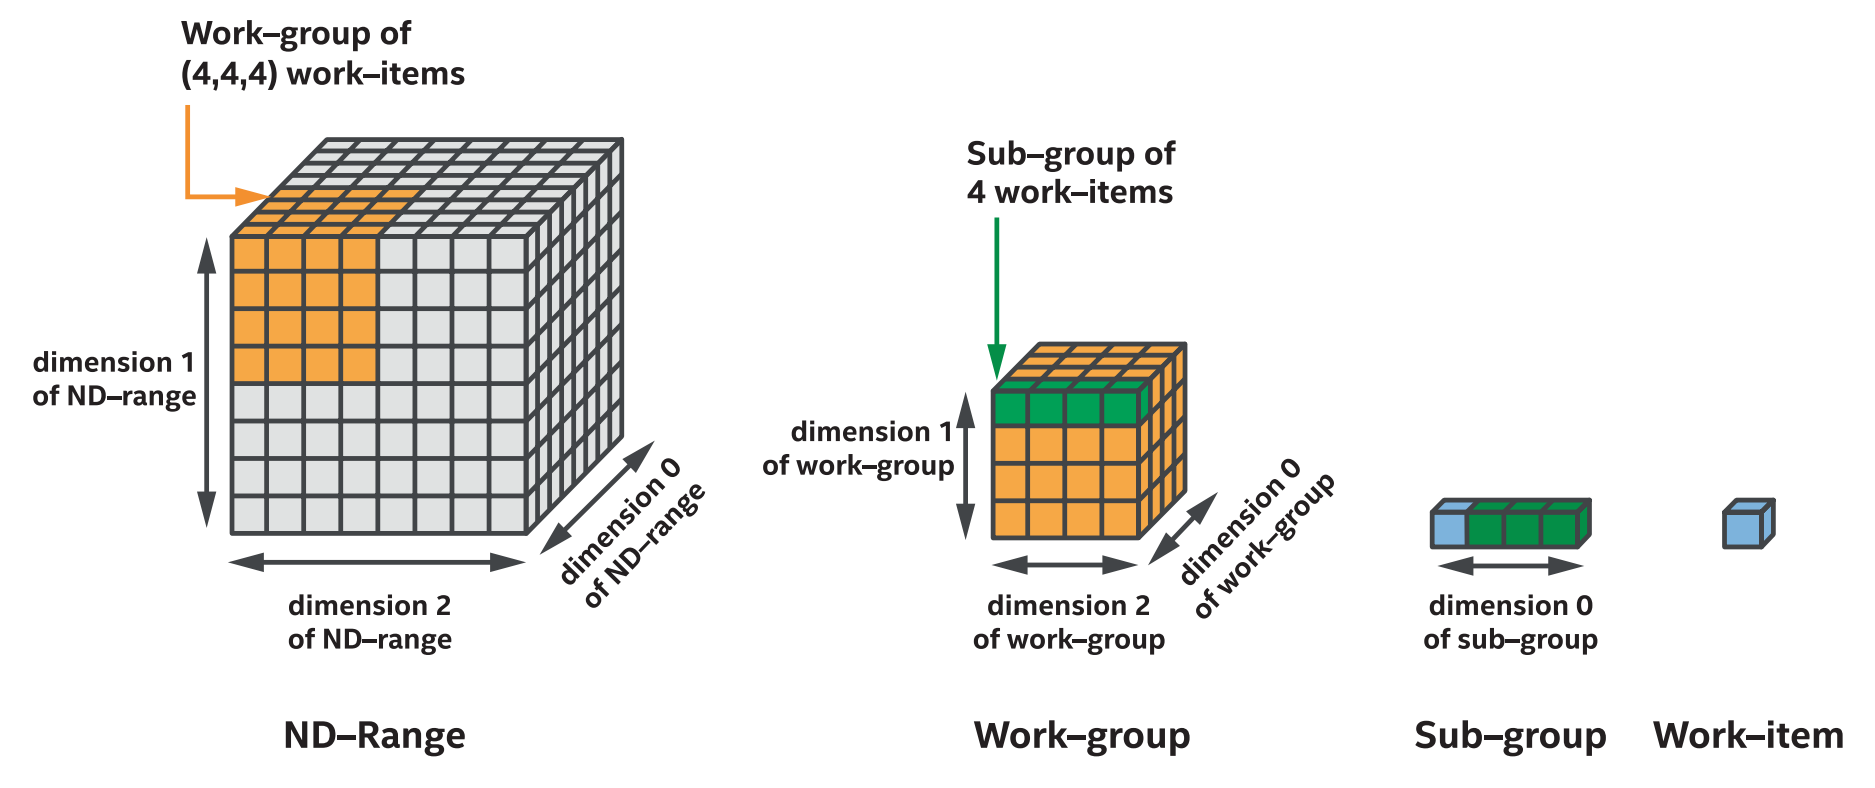
\includegraphics[width=1.0\textwidth]{content/chapter-17/images/14}
\end{center}

The FPGA spatial pipeline can be very efficiently filled with work using an ND-range. This programming style is fully supported on FPGA, and we can think of it as depicted in Figure 17-16 where on each clock cycle, a different work-item enters the first stage of the pipeline.\par

\hspace*{\fill} \par %插入空行
Figure 17-16. ND-range feeding a spatial pipeline
\begin{center}
	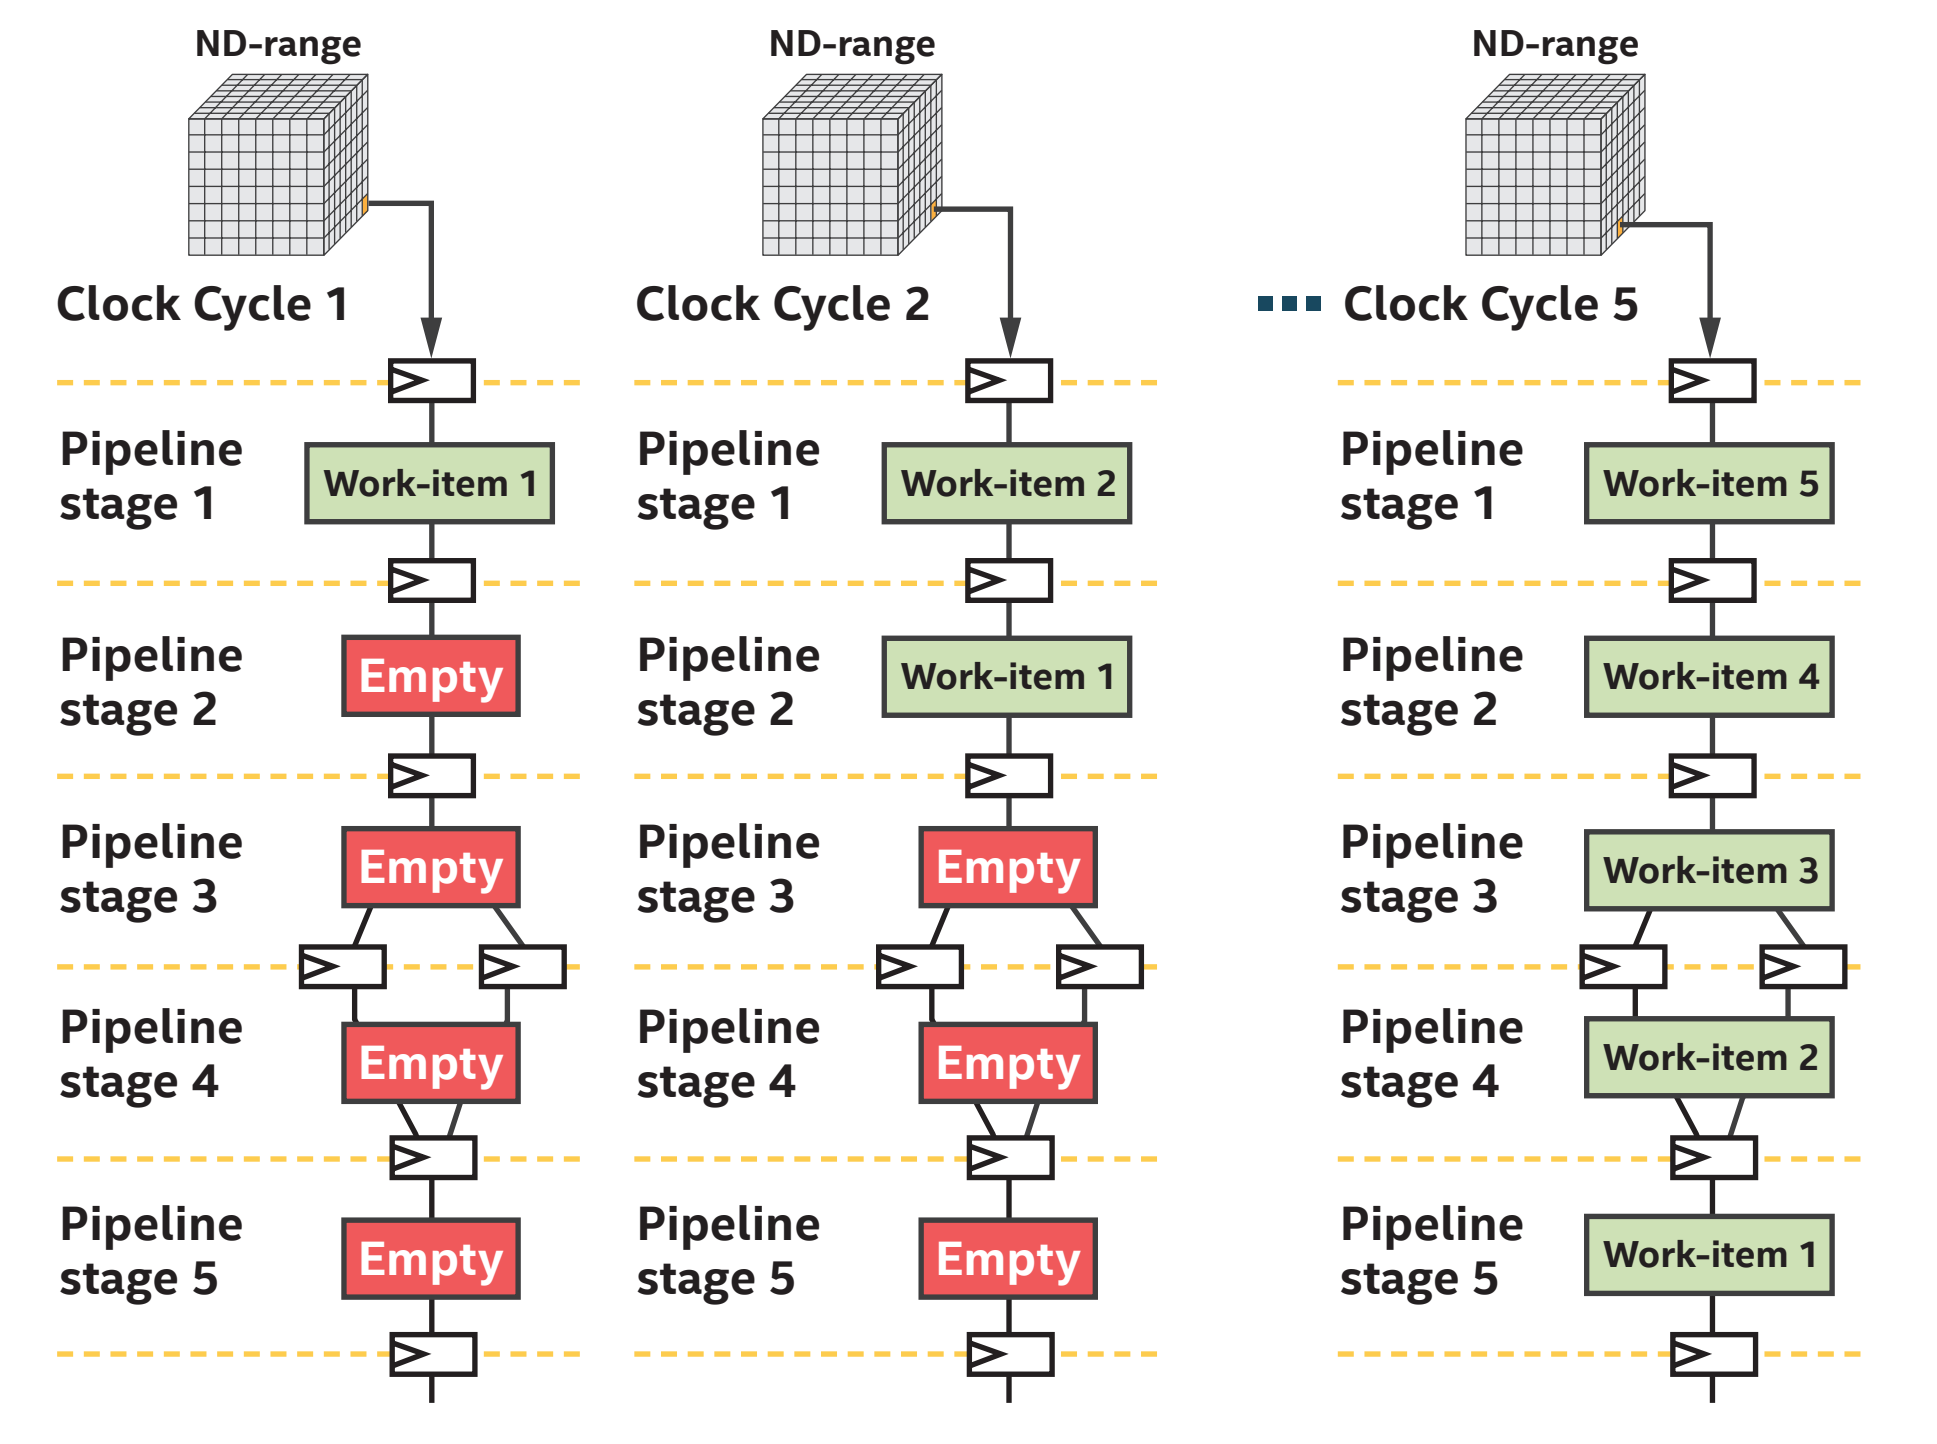
\includegraphics[width=1.0\textwidth]{content/chapter-17/images/15}
\end{center}

When should we create an ND-range kernel on an FPGA using work-items to keep the pipeline occupied? It’s simple. Whenever we can structure our algorithm or application as independent work-items that don’t need to communicate often (or ideally at all), we should use NDrange! If work-items do need to communicate often or if we don’t naturally think in terms of ND-ranges, then loops (described in the next section) provide an efficient way to express our algorithm as well.\par

\begin{tcolorbox}[colback=red!5!white,colframe=red!75!black]
If we can structure our algorithm so that work-items don’t need to communicate much (or at all), then ND-range is a great way to generate work to keep the spatial pipeline full!
\end{tcolorbox}

A good example of a kernel that is efficient with an ND-range feeding the pipeline is a random number generator, where creation of numbers in the sequence is independent of the previous numbers generated.\par

Figure 17-17 shows an ND-range kernel that will call the random number generation function once for each work-item in the 16 × 16 × 16 range. Note how the random number generation function takes the workitem id as input.\par

\hspace*{\fill} \par %插入空行
Figure 17-17. Multiple work-item (16 × 16 × 16) invocation of a random number generator
\begin{lstlisting}[caption={}]
h.parallel_for({16,16,16}, [=](auto I) {
	output[I] = generate_random_number_from_ID(I);
});
\end{lstlisting}

The example shows a parallel\_for invocation that uses a range, with only a global size specified. We can alternately use the parallel\_for invocation style that takes an nd\_range, where both the global work size and local work-group sizes are specified. FPGAs can very efficiently implement work-group local memory from on-chip resources, so feel free to use work-groups whenever they make sense, either because we want work-group local memory or because having work-group IDs available simplifies our code.\par

\begin{tcolorbox}[colback=blue!5!white,colframe=blue!75!black, title=PARALLEL RANDOM NUMBER GENERATORS]
The example in Figure 17-17 assumes that generate\_random\_number\_from\_ID(I) is a random number generator which has been written to be safe and correct when invoked in a parallel way. For example, if different work-items in the parallel\_for range execute the function, we expect different sequences to be created by each work-item, with each sequence adhering to whatever distribution is expected from the generator. Parallel random number generators are themselves a complex topic, so it is a good idea to use libraries or to learn about the topic through techniques such as block skip-ahead algorithms.
\end{tcolorbox}

\hspace*{\fill} \par %插入空行
\textbf{Pipelines Do Not Mind Data Dependences!}

One of the challenges when programming vector architectures (e.g., GPUs) where some work-items execute together as lanes of vector instructions is structuring an algorithm to be efficient without extensive communication between work-items. Some algorithms and applications lend themselves well to vector hardware, and some don’t. A common cause of a poor mapping is an algorithmic need for extensive sharing of data, due to data dependences with other computations that are in some sense neighbors. Sub-groups address some of this challenge on vector architectures by providing efficient communication between work-items in the same subgroup, as described in Chapter 14.\par

FPGAs play an important role for algorithms that can’t be decomposed into independent work. FPGA spatial pipelines are not vectorized across work-items, but instead execute consecutive work-items across pipeline stages. This implementation of the parallelism means that fine-grained communication between work-items (even those in different work-groups) can be implemented easily and efficiently within the spatial pipeline!\par

One example is a random number generator where output N+1 depends on knowing what output N was. This creates a data dependence between two outputs, and if each output is generated by a work-item in an ND-range, then there is a data dependence between work-items that can require complex and often costly synchronization on some architectures. When coding such algorithms serially, one would typically write a loop, where iteration N+1 uses the computation from iteration N, such as shown in Figure 17-18. Each iteration depends on the state computed by the previous iteration. This is a very common pattern.\par

\hspace*{\fill} \par %插入空行
Figure 17-18. Loop-carried data dependence (state)
\begin{lstlisting}[caption={}]
int state = 0;
for (int i=0; i < size; i++) {
	state = generate_random_number(state);
	output[i] = state;
}
\end{lstlisting}

Spatial implementations can very efficiently communicate results backward in the pipeline to work that started in a later cycle (i.e., to work at an earlier stage in the pipeline), and spatial compilers implement many optimizations around this pattern. Figure 17-19 shows the idea of backward communication of data, from stage 5 to stage 4. Spatial pipelines are not vectorized across work-items. This enables efficient data dependence communication by passing results backward in the pipeline!\par

\hspace*{\fill} \par %插入空行
Figure 17-19. Backward communication enables efficient data dependence communication
\begin{center}
	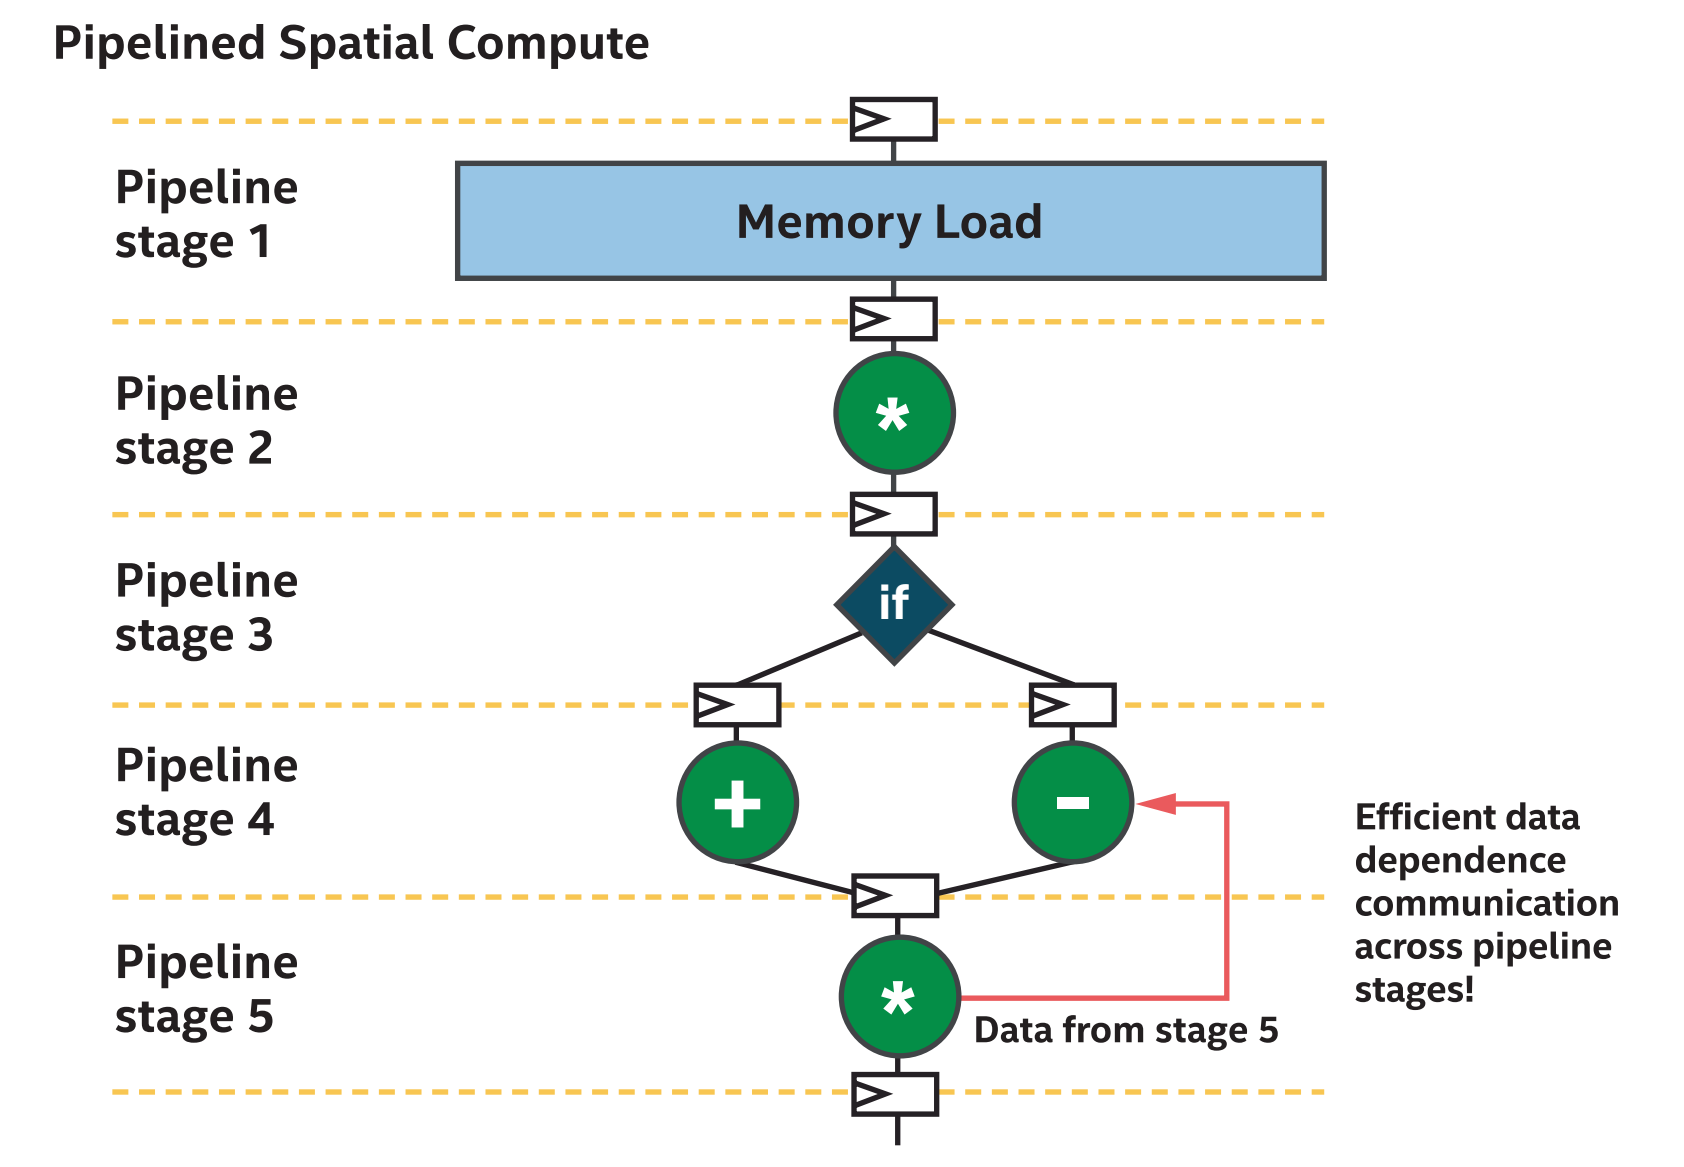
\includegraphics[width=1.0\textwidth]{content/chapter-17/images/16}
\end{center}

The ability to pass data backward (to an earlier stage in the pipeline) is key to spatial architectures, but it isn’t obvious how to write code that takes advantage of it. There are two approaches that make expressing this pattern easy:\par

\begin{enumerate}
	\item Loops
	\item Intra-kernel pipes with ND-range kernels
\end{enumerate}

The second option is based on pipes that we describe later in this chapter, but it isn’t nearly as common as loops so we mention it for completeness, but don’t detail it here. Vendor documentation provides more details on the pipe approach, but it’s easier to stick to loops which are described next unless there is a reason to do otherwise.\par

\hspace*{\fill} \par %插入空行
\textbf{Spatial Pipeline Implementation of a Loop}

A loop is a natural fit when programming an algorithm that has data dependences. Loops frequently express dependences across iterations, even in the most basic loop examples where the counter that determines when the loop should exit is carried across iterations (variable i in Figure 17-20).\par

\hspace*{\fill} \par %插入空行
Figure 17-20. Loop with two loop-carried dependences (i.e., i and a)
\begin{lstlisting}[caption={}]
int a = 0;
for (int i=0; i < size; i++) {
	a = a + i;
}
\end{lstlisting}

In the simple loop of Figure 17-20, it is understood that the value of a which is on the right-hand side of a= a + i reflects the value stored by the previous loop iteration or the initial value if it’s the first iteration of the loop. When a spatial compiler implements a loop, iterations of the loop can be used to fill the stages of the pipeline as shown in Figure 17-21. Notice that the queue of work which is ready to start now contains loop iterations, not work-items!\par

\hspace*{\fill} \par %插入空行
Figure 17-21. Pipelines stages fed by successive iterations of a loop
\begin{center}
	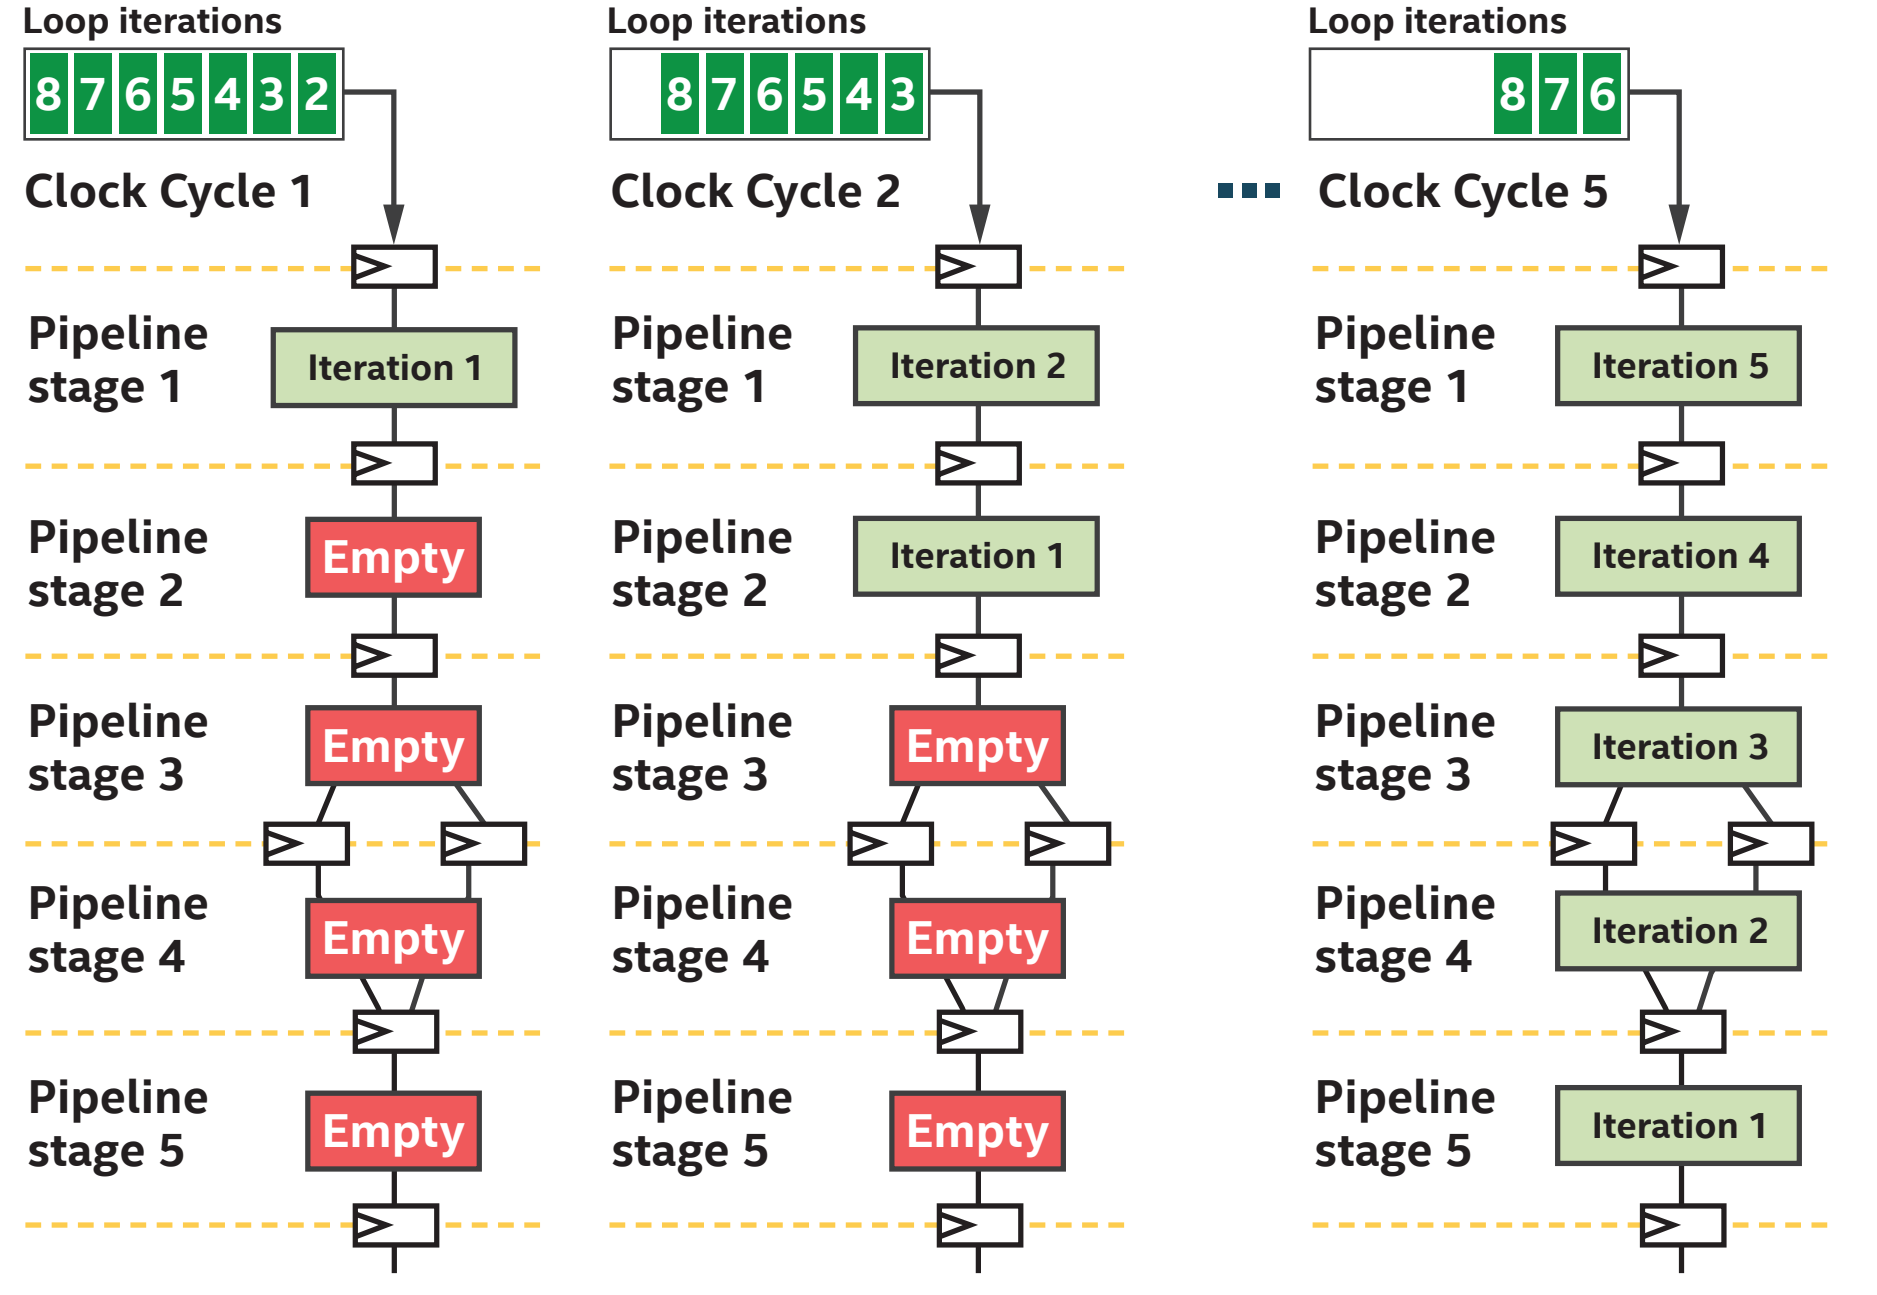
\includegraphics[width=1.0\textwidth]{content/chapter-17/images/17}
\end{center}

A modified random number generator example is shown in Figure 17-22. In this case, instead of generating a number based on the id of a work-item, as in Figure 17-17, the generator takes the previously computed value as an argument.\par

\hspace*{\fill} \par %插入空行
Figure 17-22. Random number generator that depends on previous value generated
\begin{lstlisting}[caption={}]
h.single_task([=]() {
	int state = seed;
	for (int i=0; i < size; i++) {
		state = generate_incremental_random_number(state);
		output[i] = state;
	}
});
\end{lstlisting}

The example uses single\_task instead of parallel\_for because the repeated work is expressed by a loop within the single task, so there isn’t a reason to also include multiple work-items in this code (via parallel\_for). The loop inside the single\_task makes it much easier to express (programming convenience) that the previously computed value of temp is passed to each invocation of the random number generation function.\par

In cases such as Figure 17-22, the FPGA can implement the loop efficiently. It can maintain a fully occupied pipeline in many cases or can at least tell us through reports what to change to increase occupancy. With this in mind, it becomes clear that this same algorithm would be much more difficult to describe if loop iterations were replaced with work-items, where the value generated by one work-item would need to be communicated to another work-item to be used in the incremental computation. The code complexity would rapidly increase, particularly if the work couldn’t be batched so that each work-item was actually computing its own independent random number sequence.\par

\hspace*{\fill} \par %插入空行
\textbf{Loop Initiation Interval}

Conceptually, we probably think of iterations of a loop in C++ as executing one after another, as shown in Figure 17-23. That’s the programming model and is the right way to think about loops. In implementation, though, compilers are free to perform many optimizations as long as most behavior (i.e., defined and race-free behavior) of the program doesn’t observably change. Regardless of compiler optimizations, what matters is that the loop appears to execute as if Figure 17-23 is how it happened.\par

\hspace*{\fill} \par %插入空行
Figure 17-23. Conceptually, loop iterations execute one after anothe
\begin{center}
	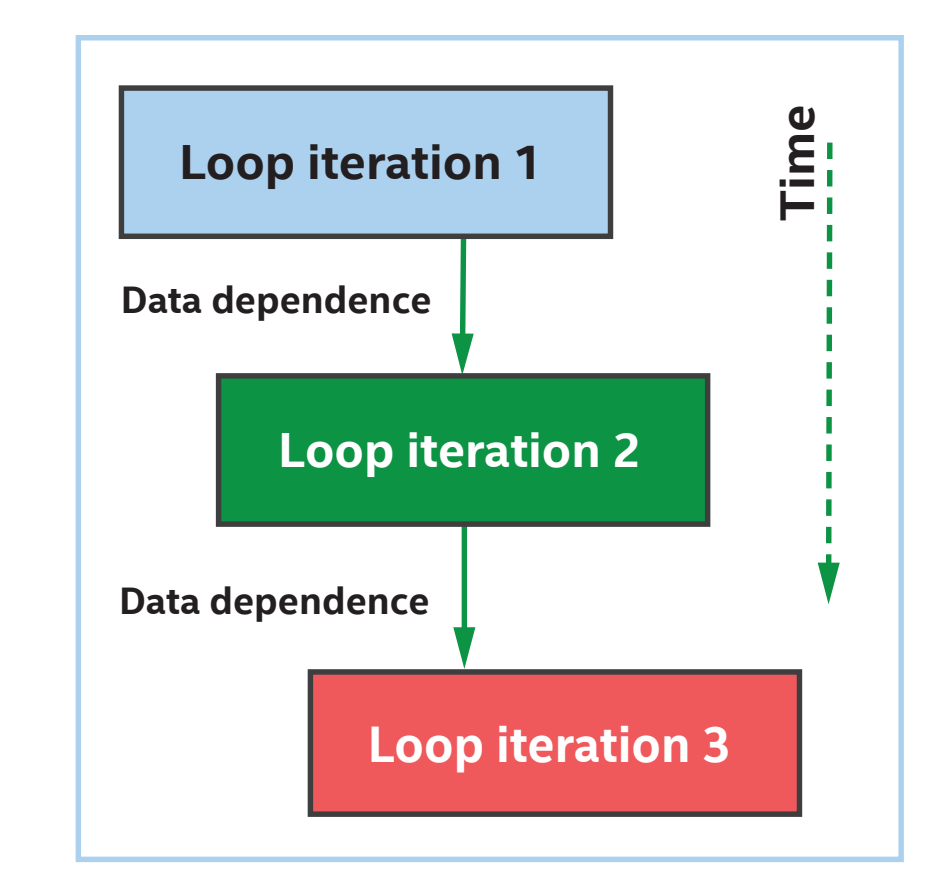
\includegraphics[width=1.0\textwidth]{content/chapter-17/images/18}
\end{center}

Moving into the spatial compiler perspective, Figure 17-24 shows a loop pipelining optimization where the execution of iterations of a loop are overlapped in time. Different iterations will be executing different stages of the spatial pipeline from each other, and data dependences across stages of the pipeline can be managed by the compiler to ensure that the program appears to execute as if the iterations were sequential (except that the loop will finish executing sooner!).\par

\hspace*{\fill} \par %插入空行
Figure 17-24. Loop pipelining allows iterations of the loop to be overlapped across pipeline stages
\begin{center}
	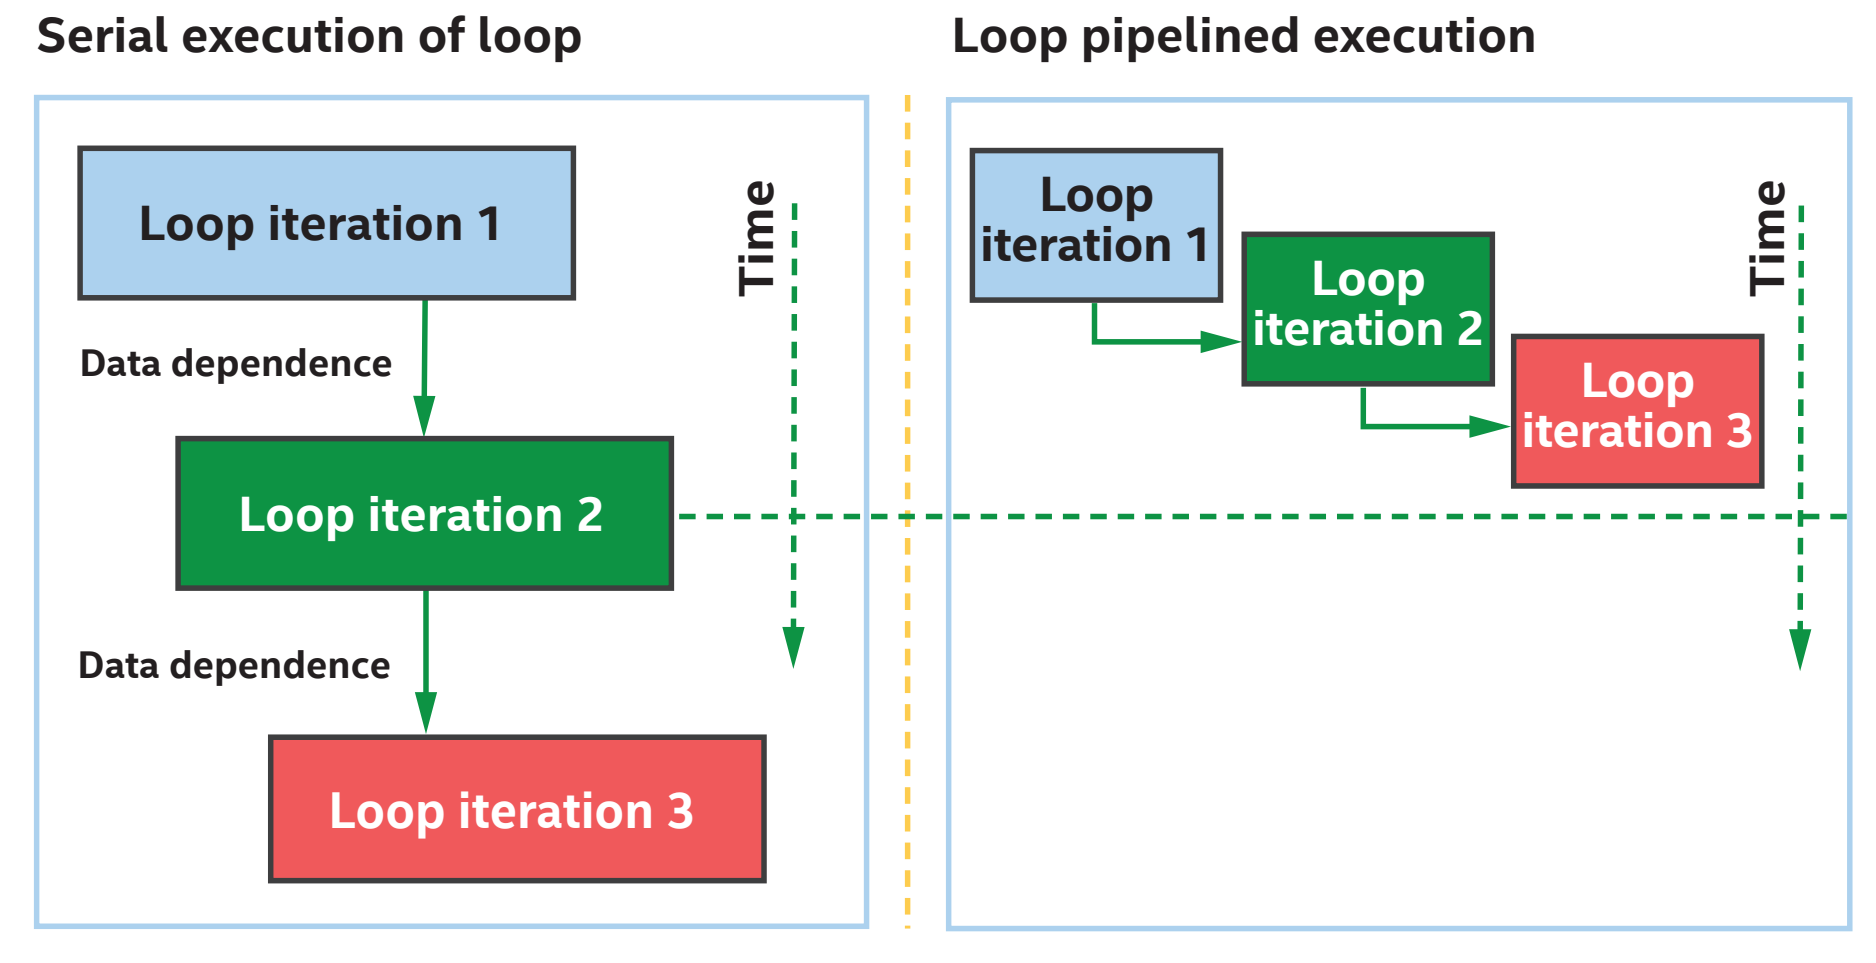
\includegraphics[width=1.0\textwidth]{content/chapter-17/images/19}
\end{center}

Loop pipelining is easy to understand with the realization that many results within a loop iteration may finish computation well before the loop iteration finishes all of its work and that, in a spatial pipeline, results can be passed to an earlier pipeline stage when the compiler decides to do so. Figure 17-25 shows this idea where the results of stage 1 are fed backward in the pipeline, allowing a future loop iteration to use the result early, before the previous iteration has completed.\par

\hspace*{\fill} \par %插入空行
Figure 17-25. A pipelined implementation of the incremental random number generator
\begin{center}
	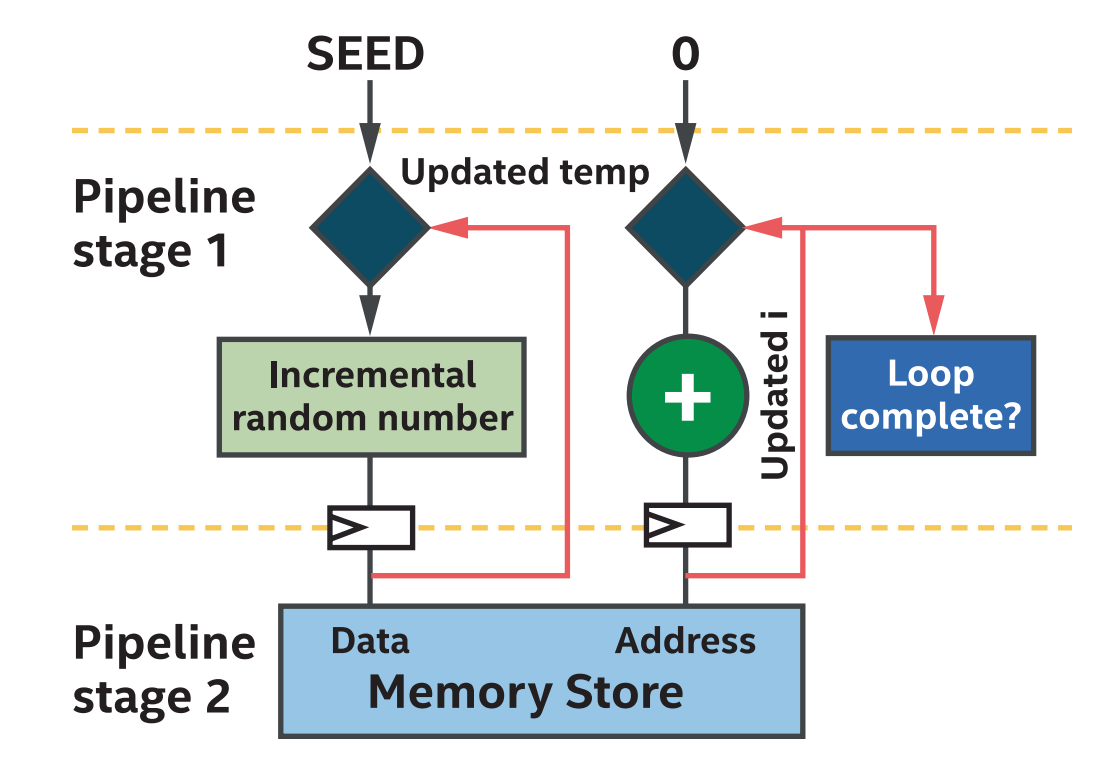
\includegraphics[width=1.0\textwidth]{content/chapter-17/images/20}
\end{center}

With loop pipelining, it is possible for the execution of many iterations of a loop to overlap. The overlap means that even with loop-carried data dependences, loop iterations can still be used to fill the pipeline with work, leading to efficient utilization. Figure 17-26 shows how loop iterations might overlap their executions, even with loop-carried data dependences, within the same simple pipeline as was shown in Figure 17-25.\par

\hspace*{\fill} \par %插入空行
Figure 17-26. Loop pipelining simultaneously processes parts of multiple loop iterations
\begin{center}
	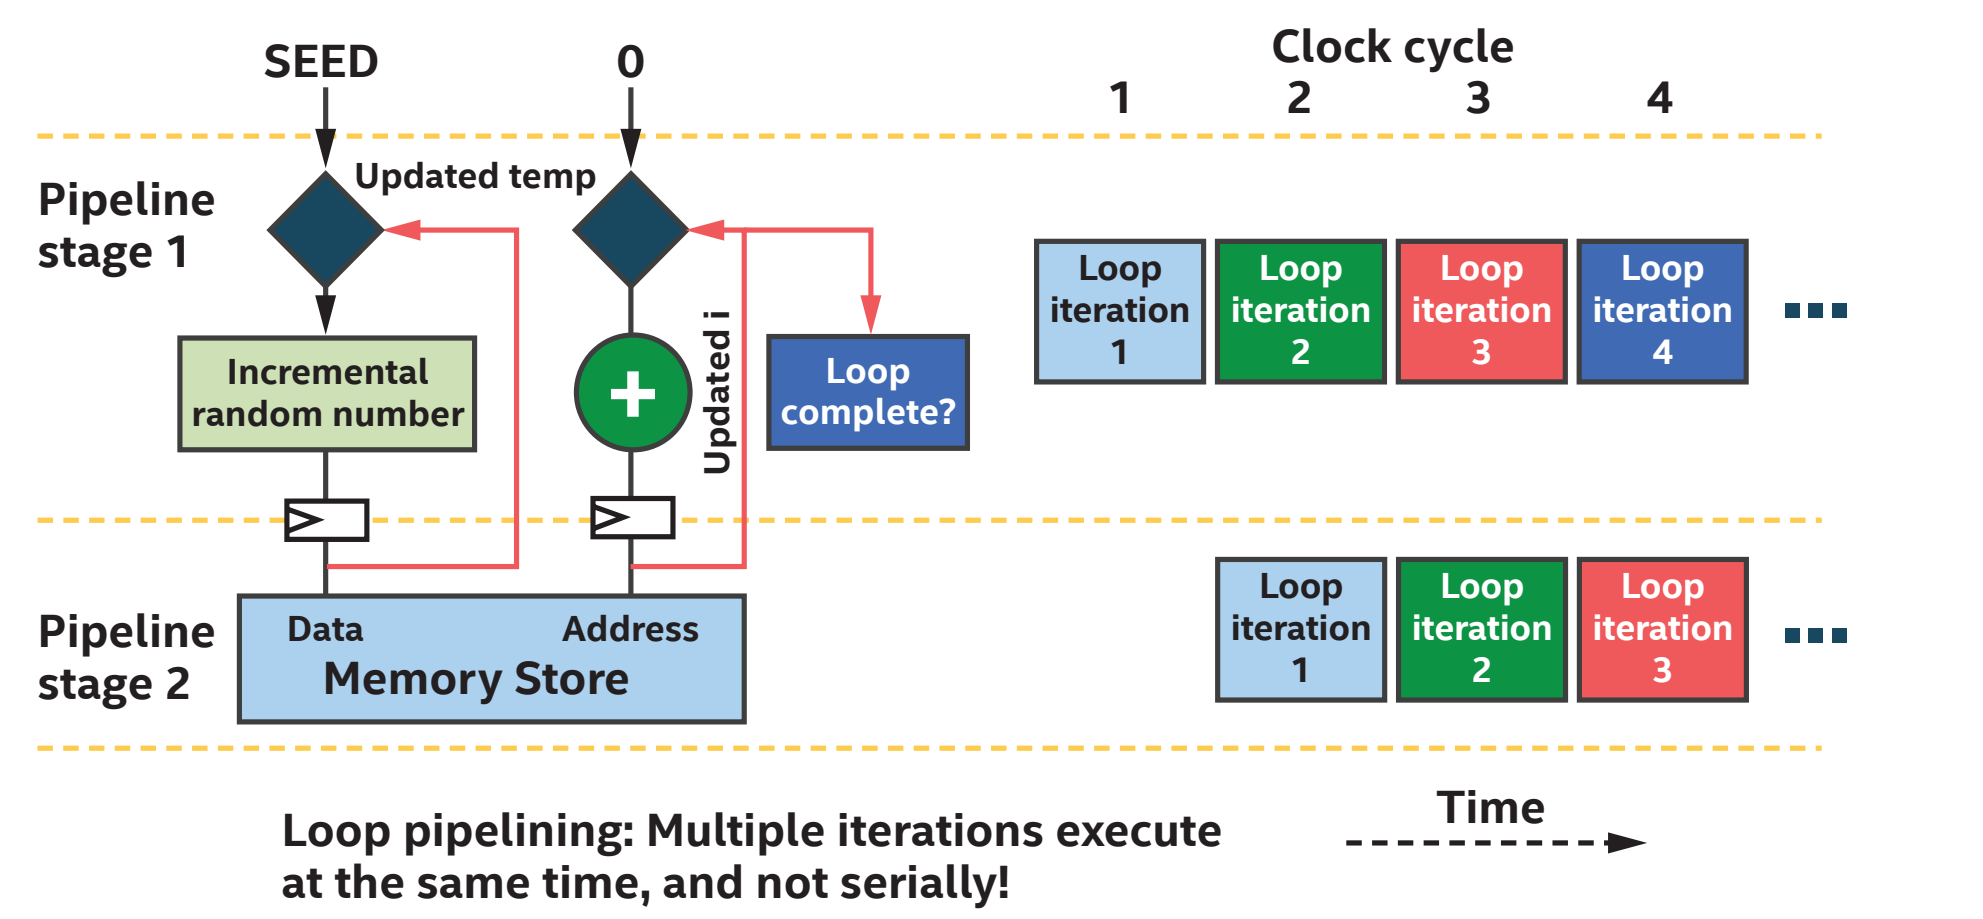
\includegraphics[width=1.0\textwidth]{content/chapter-17/images/21}
\end{center}

In real algorithms, it is often not possible to launch a new loop iteration every single clock cycle, because a data dependence may take multiple clock cycles to compute. This often arises if memory lookups, particularly from off-chip memories, are on the critical path of the computation of a dependence. The result is a pipeline that can only initiate a new loop iteration every N clock cycles, and we refer to this as an initiation interval(II) of N cycles. An example is shown in Figure 17-27. A loop initiation interval (II) of two means that a new loop iteration can begin every second cycle, which results in sub-optimal occupancy of the pipeline stages.\par

\hspace*{\fill} \par %插入空行
Figure 17-27. Sub-optimal occupancy of pipeline stages
\begin{center}
	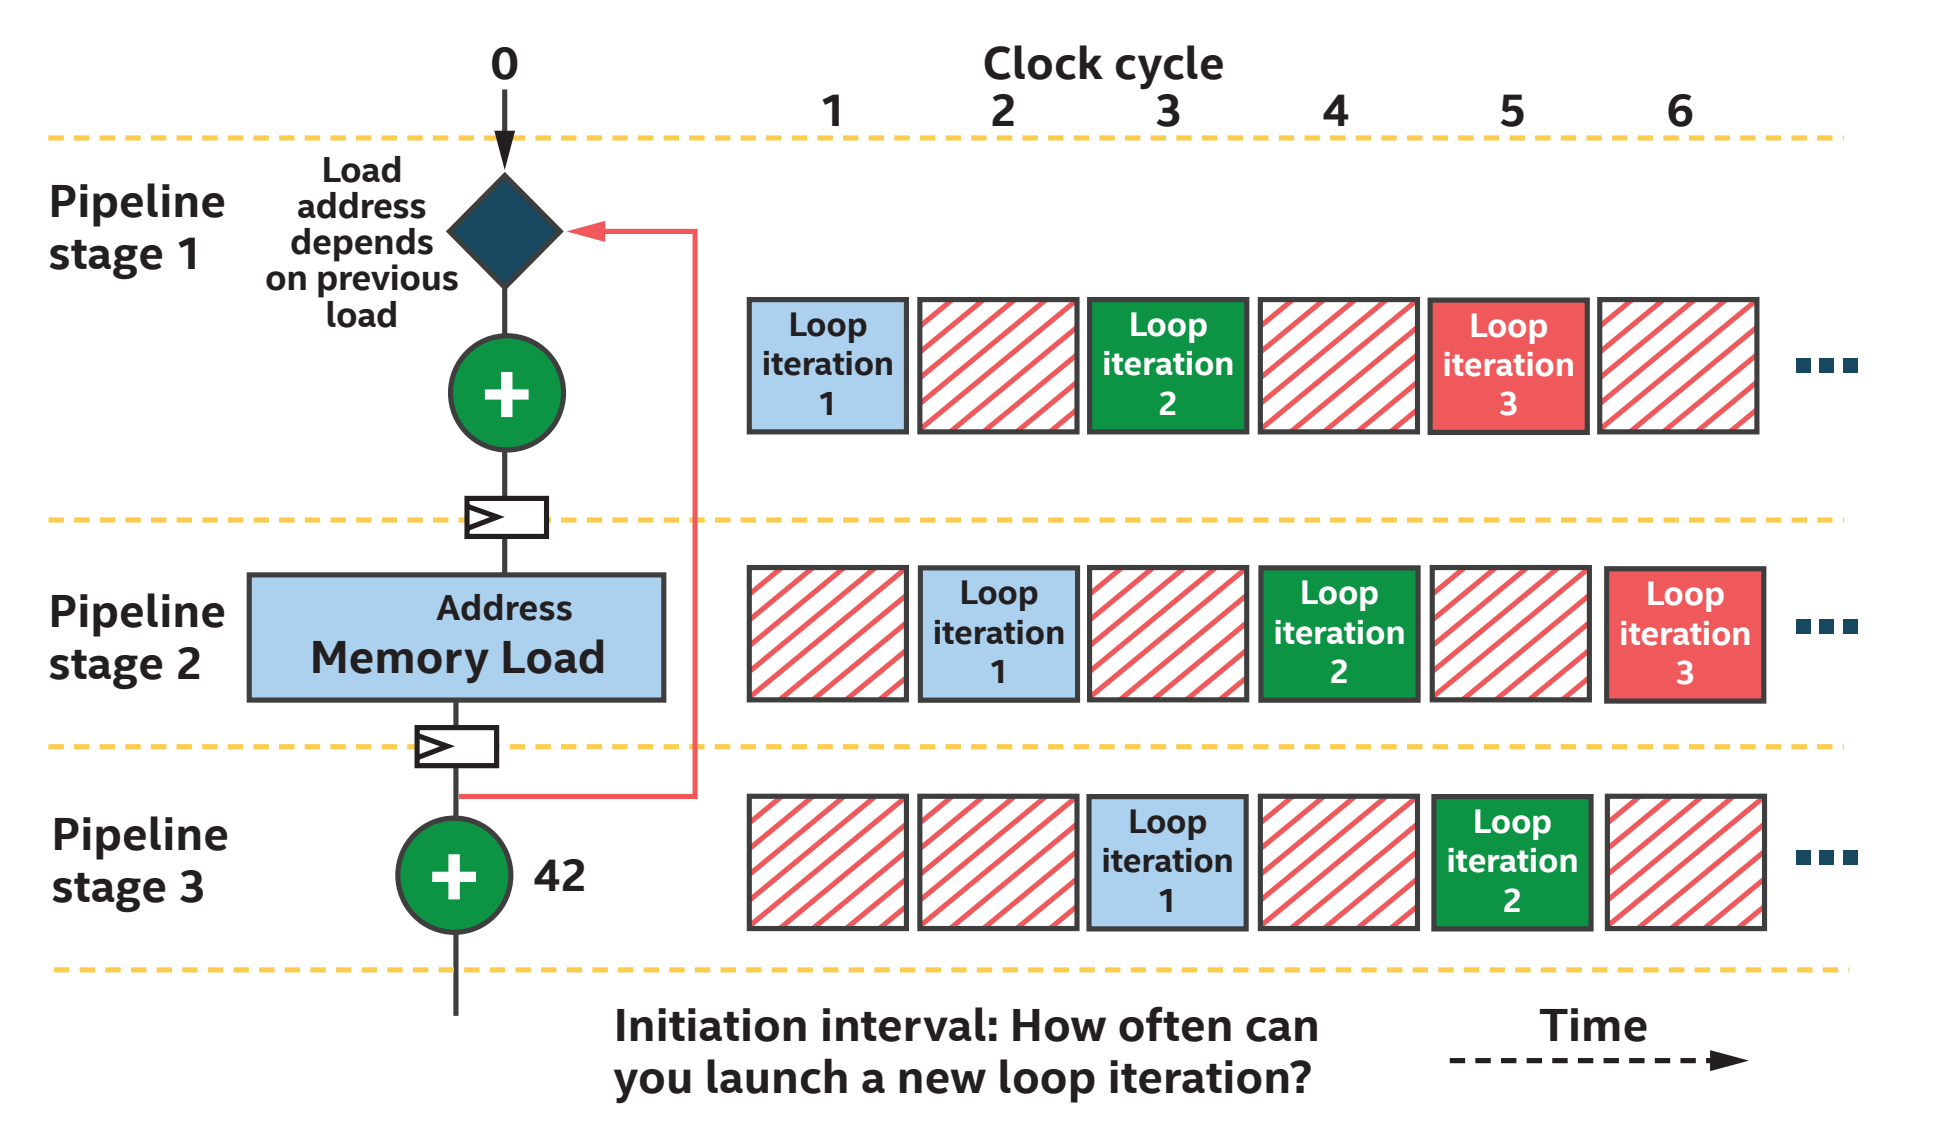
\includegraphics[width=1.0\textwidth]{content/chapter-17/images/22}
\end{center}

An II larger than one can lead to inefficiency in the pipeline because the average occupancy of each stage is reduced. This is apparent from Figure 17-27 where II=2 and pipeline stages are unused a large percentage (50\%!) of the time. There are multiple ways to improve this situation.\par

The compiler performs extensive optimization to reduce II whenever possible, so its reports will also tell us what the initiation interval of each loop is and give us information on why it is larger than one, if that occurs. Restructuring the compute in a loop based on the reports can often reduce the II, particularly because as developers, we can make loop structural changes that the compiler isn’t allowed to (because they would be observable). Read the compiler reports to learn how to reduce the II in specific cases.\par

An alternative way to reduce inefficiency from an II that is larger than one is through nested loops, which can fill all pipeline stages through interleaving of outer loop iterations with those of an inner loop that has II>1. Check vendor documentation and the compiler reports for details on using this technique.\par

\hspace*{\fill} \par %插入空行
\textbf{Pipes}

An important concept in spatial and other architectures is a first-in firstout (FIFO) buffer. There are many reasons that FIFOs are important, but two properties are especially useful when thinking about programming:\par

\begin{enumerate}
	\item There is implicit control information carried alongside the data. These signals tell us whether the FIFO is empty or full and can be useful when decomposing a problem into independent pieces.
	\item FIFOs have storage capacity. This can make it easier to achieve performance in the presence of dynamic behaviors such as highly variable latencies when accessing memory
\end{enumerate}

Figure 17-28 shows a simple example of a FIFO’s operation.\par

\hspace*{\fill} \par %插入空行
Figure 17-28. Example operation of a FIFO over time
\begin{center}
	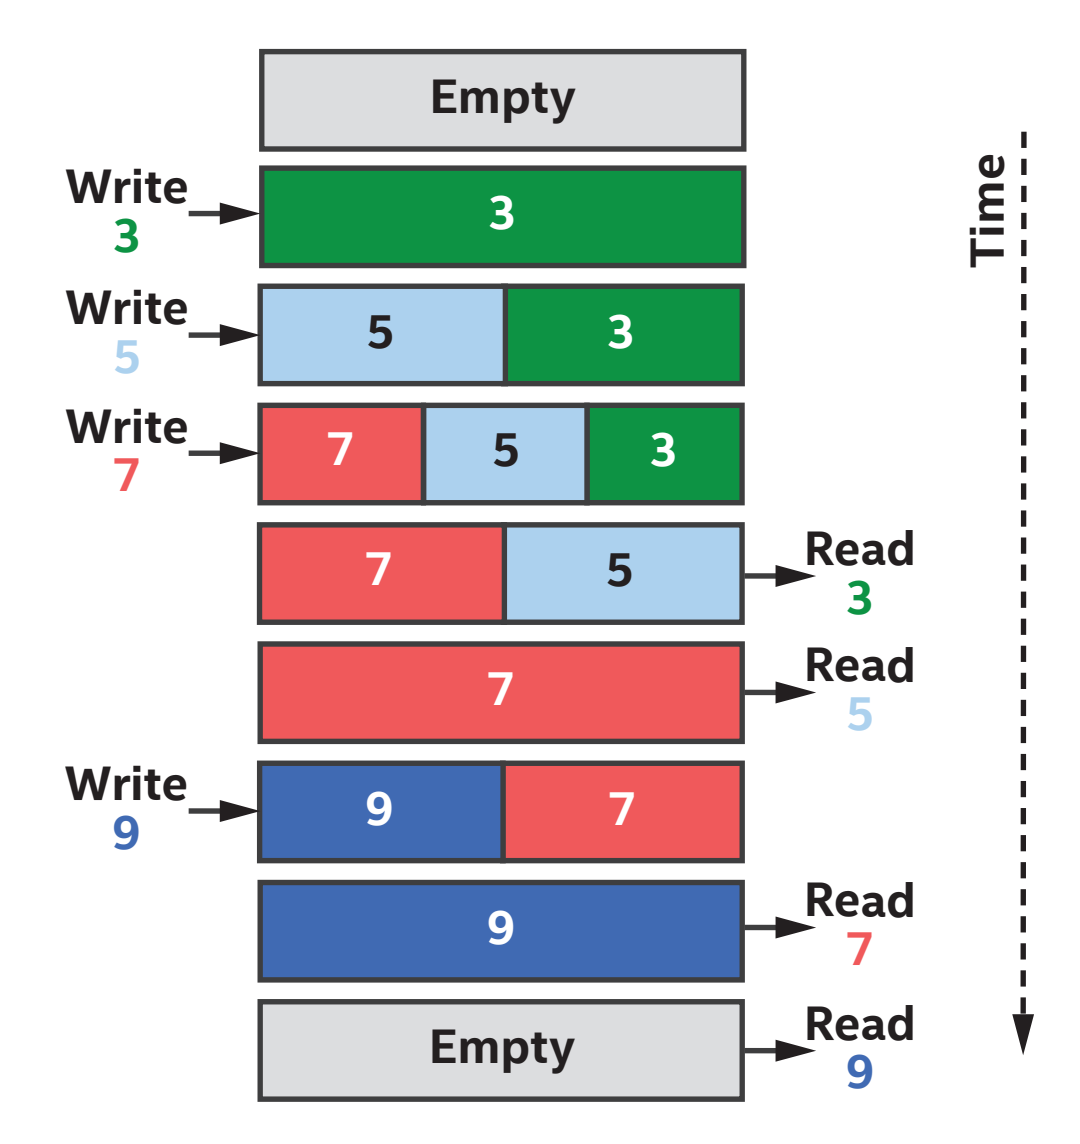
\includegraphics[width=1.0\textwidth]{content/chapter-17/images/23}
\end{center}

FIFOs are exposed in DPC++ through a feature called pipes. The main reason that we should care about pipes when writing FPGA programs is that they allow us to decompose a problem into smaller pieces to focus on development and optimizations in a more modular way. They also allow the rich communication features of the FPGA to be harnessed. Figure 17-29 shows both of these graphically.\par

\hspace*{\fill} \par %插入空行
Figure 17-29. Pipes simplify modular design and access to hardware peripherals
\begin{center}
	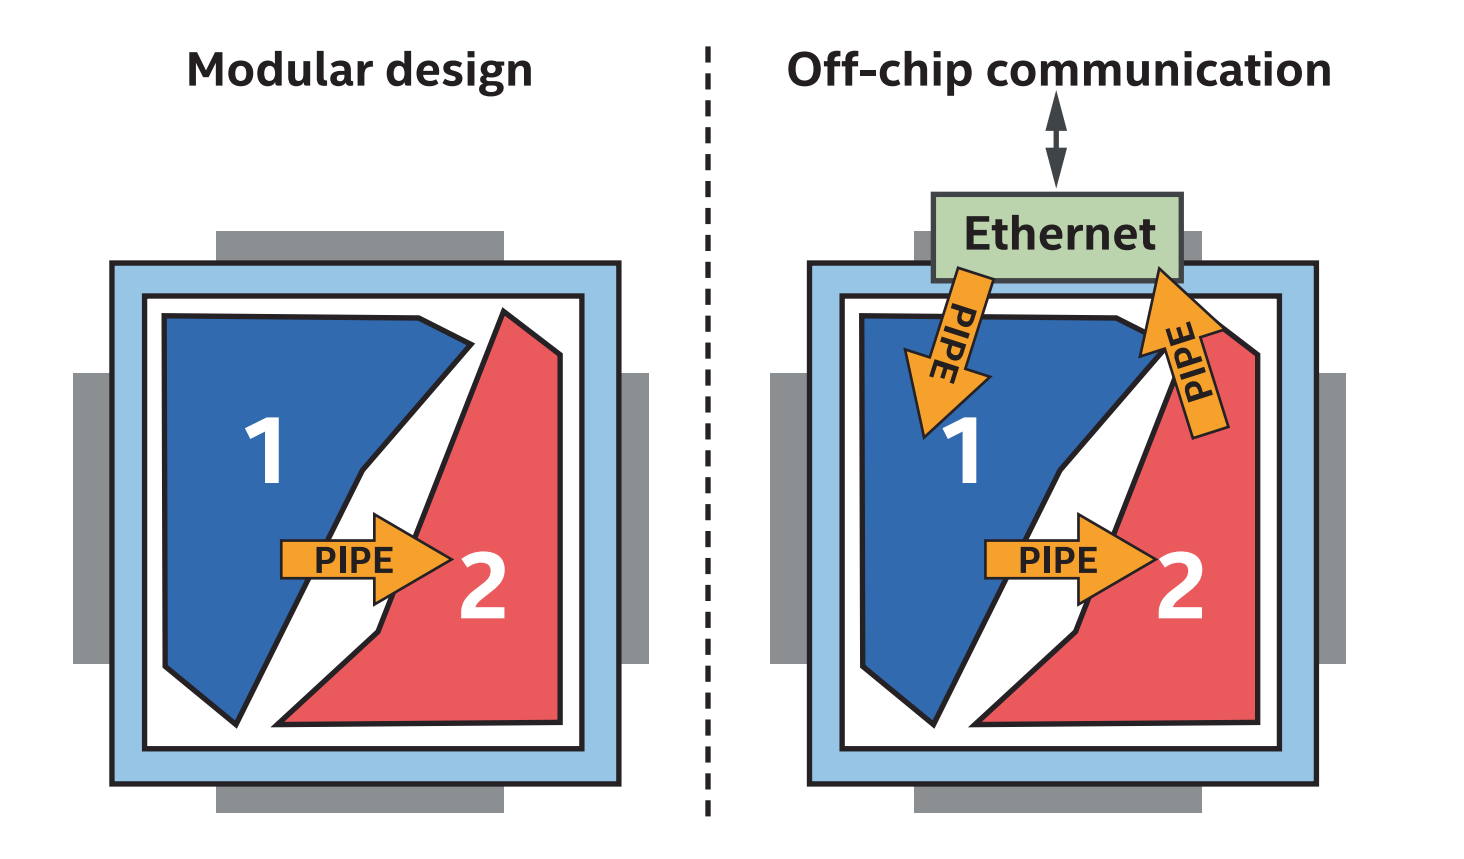
\includegraphics[width=1.0\textwidth]{content/chapter-17/images/24}
\end{center}

Remember that FPGA kernels can exist on the device simultaneously (in different areas of the chip) and that in an efficient design, all parts of the kernels are active all the time, every clock cycle. This means that optimizing an FPGA application involves considering how kernels or parts of kernels interact with one another, and pipes provide an abstraction to make this easy.\par

Pipes are FIFOs that are implemented using on-chip memories on an FPGA, so they allow us to communicate between and within running kernels without the cost of moving data to off-chip memory. This provides inexpensive communication, and the control information that is coupled with a pipe (empty/full signals) provides a lightweight synchronization mechanism.\par

\begin{tcolorbox}[colback=blue!5!white,colframe=blue!75!black, title=DO WE NEED PIPES?]
No. It is possible to write efficient kernels without using pipes. We can use all of the FPGA resources and achieve maximum performance using conventional programming styles without pipes. But it is easier for most developers to program and optimize more modular spatial designs, and pipes are a great way to achieve this.
\end{tcolorbox}

As shown in Figure 17-30, there are four general types of pipes available. In the rest of this section, we’ll cover the first type (inter-kernel pipes), because they suffice to show what pipes are and how they are used. Pipes can also communicate within a single kernel and with the host or input/output peripherals. Please check vendor documentation for more information on those forms and uses of pipes that we don’t have room to dive into here.\par

\hspace*{\fill} \par %插入空行
Figure 17-30. Types of pipe connectivity in DPC++
\begin{center}
	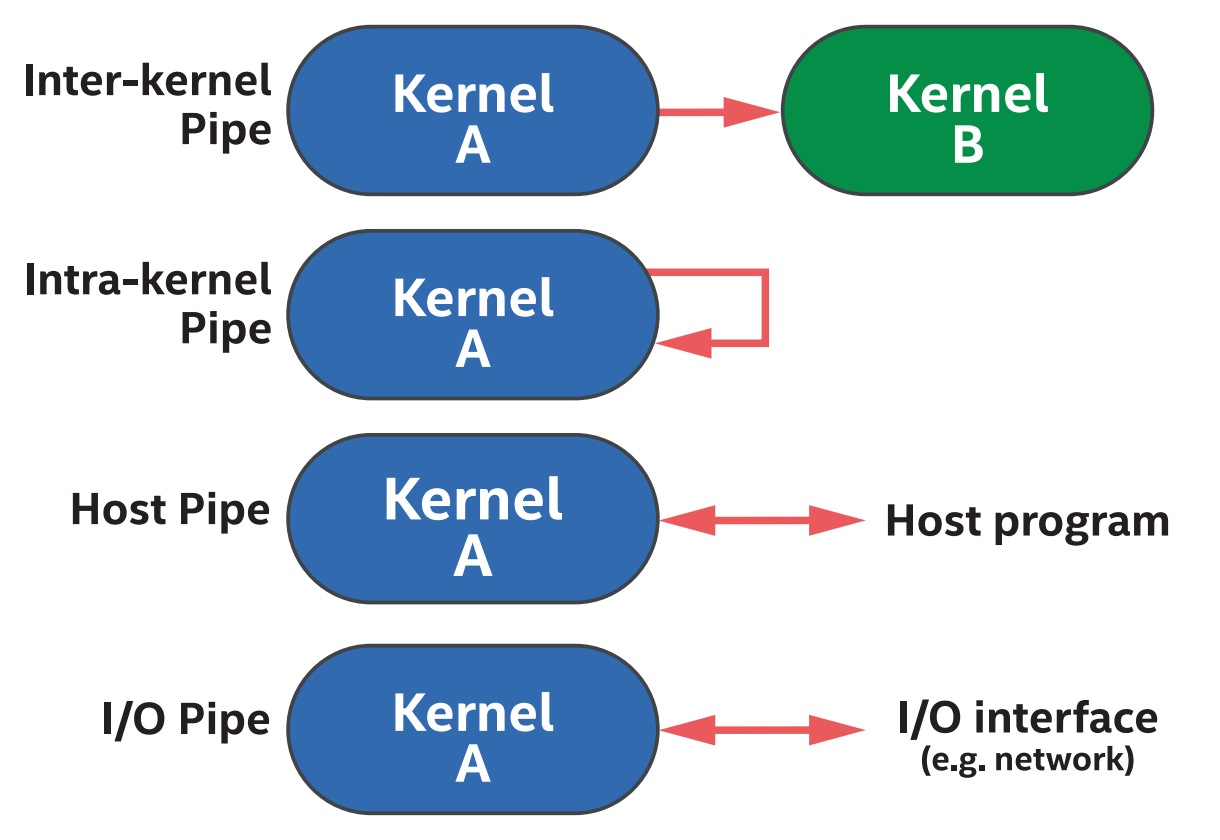
\includegraphics[width=1.0\textwidth]{content/chapter-17/images/25}
\end{center}

A simple example is shown in Figure 17-31. In this case, there are two kernels that communicate through a pipe, with each read or write operating on a unit of an int.\par

\hspace*{\fill} \par %插入空行
Figure 17-31. Pipe between two kernels: (1) ND-range and (2) single task with a loop
\begin{lstlisting}[caption={}]
// Create alias for pipe type so that consistent across uses
using my_pipe = pipe<class some_pipe, int>;

// ND-range kernel
Q.submit([&](handler& h) {
	auto A = accessor(B_in, h);
	
	h.parallel_for(count, [=](auto idx) {
		my_pipe::write( A[idx] );
	});
});

// Single_task kernel
Q.submit([&](handler& h) {
	auto A = accessor(B_out, h);
	
	h.single_task([=]() {
		for (int i=0; i < count; i++) {
			A[i] = my_pipe::read();
		}
	});
});
\end{lstlisting}

There are a few points to observe from Figure 17-31. First, two kernels are communicating with each other using a pipe. If there are no accessor or event dependences between the kernels, the DPC++ runtime will execute both at the same time, allowing them to communicate through the pipe instead of full SYCL memory buffers or USM.\par

Pipes are identified using a type-based approach, where each is identified using a parameterization of the pipe type which is shown in Figure 17-32. The parameterization of the pipe type identifies a specific pipe. Reads or writes on the same pipe type are to the same FIFO. There are three template parameters that together define the type and therefore identity of a pipe.\par

\hspace*{\fill} \par %插入空行
Figure 17-32. Parameterization of the pipe type
\begin{lstlisting}[caption={}]
template <typename name,
		  typename dataT,
		  size_t min_capacity = 0>
class pipe;
\end{lstlisting}

It is recommended to use type aliases to define our pipe types, as shown in the first line of code in Figure 17-31, to reduce programming errors and improve code readability.\par

\begin{tcolorbox}[colback=red!5!white,colframe=red!75!black]
Use type aliases to identify pipes. This simplifies code and prevents accidental creation of unexpected pipes.
\end{tcolorbox}

Pipes have a min\_capacity parameter. It defaults to 0 which is automatic selection, but if specified, it guarantees that at least that number of words can be written to the pipe without any being read out. This parameter is useful when\par

\begin{enumerate}
	\item Two kernels communicating with a pipe do not run at the same time, and we need enough capacity in the pipe for a first kernel to write all of its outputs before a second kernel starts to run and reads from the pipe.
	\item If kernels generate or consume data in bursts, then adding capacity to a pipe can provide isolation between the kernels, decoupling their performance from each other. For example, a kernel producing data can continue to write (until the pipe capacity becomes full), even if a kernel consuming that data is busy and not ready to consume anything yet. This provides flexibility in execution of kernels relative to each other, at the cost only of some memory resources on the FPGA.
\end{enumerate}

\hspace*{\fill} \par %插入空行
\textbf{Blocking and Non-blocking Pipe Accesses}

Like most FIFO interfaces, pipes have two styles of interface: blocking and non-blocking. Blocking accesses wait (block/pause execution!) for the operation to succeed, while non-blocking accesses return immediately and set a Boolean value indicating whether the operation succeeded.\par

The definition of success is simple: If we are reading from a pipe and there was data available to read (the pipe wasn’t empty), then the read succeeds. If we are writing and the pipe wasn’t already full, then the write succeeds. Figure 17-33 shows both forms of access member functions of the pipe class. We see the member functions of a pipe that allow it to be written to or read from. Recall that accesses to pipes can be blocking or non-blocking.\par

\hspace*{\fill} \par %插入空行
Figure 17-33. Member functions of a pipe that allow it to be written to or read from
\begin{lstlisting}[caption={}]
// Blocking
T read();
void write( const T &data );

// Non-blocking
T read( bool &success_code );
void write( const T &data, bool &success_code ); 
\end{lstlisting}

Both blocking and non-blocking accesses have their uses depending on what our application is trying to achieve. If a kernel can’t do any more work until it reads data from the pipe, then it probably makes sense to use a blocking read. If instead a kernel wants to read data from any one of a set of pipes and it is not sure which one might have data available, then reading from pipes with a non-blocking call makes more sense. In that case, the kernel can read from a pipe and process the data if there was any, but if the pipe was empty, it can instead move on and try reading from the next pipe that potentially has data available.\par

\hspace*{\fill} \par %插入空行
\textbf{For More Information on Pipes}

We could only scratch the surface of pipes in this chapter, but we should now have an idea of what they are and the basics of how to use them. FPGA vendor documentation has a lot more information and many examples of their use in different types of applications, so we should look there if we think that pipes are relevant for our particular needs.\par

\hspace*{\fill} \par %插入空行
\textbf{Custom Memory Systems}

When programming for most accelerators, much of the optimization effort tends to be spent making memory accesses more efficient. The same is true of FPGA designs, particularly when input and output data pass through off-chip memory.\par

There are two main reasons that memory accesses on an FPGA can be worth optimizing:\par

\begin{enumerate}
	\item To reduce required bandwidth, particularly if some of that bandwidth is used inefficiently
	\item To modify access patterns on a memory that is leading to unnecessary stalls in the spatial pipeline
\end{enumerate}

It is worth talking briefly about stalls in the spatial pipeline. The compiler builds in assumptions about how long it will take to read from or write to specific types of memories, and it optimizes and balances the pipeline accordingly, hiding memory latencies in the process. But if we access memory in an inefficient way, we can introduce longer latencies and as a by-product stalls in the pipeline, where earlier stages cannot make progress executing because they’re blocked by a pipeline stage that is waiting for something (e.g., a memory access). Figure 17-34 shows such a situation, where the pipeline above the load is stalled and unable to make forward progress.\par

\hspace*{\fill} \par %插入空行
Figure 17-34. How a memory stall can cause earlier pipeline stages to stall as well
\begin{center}
	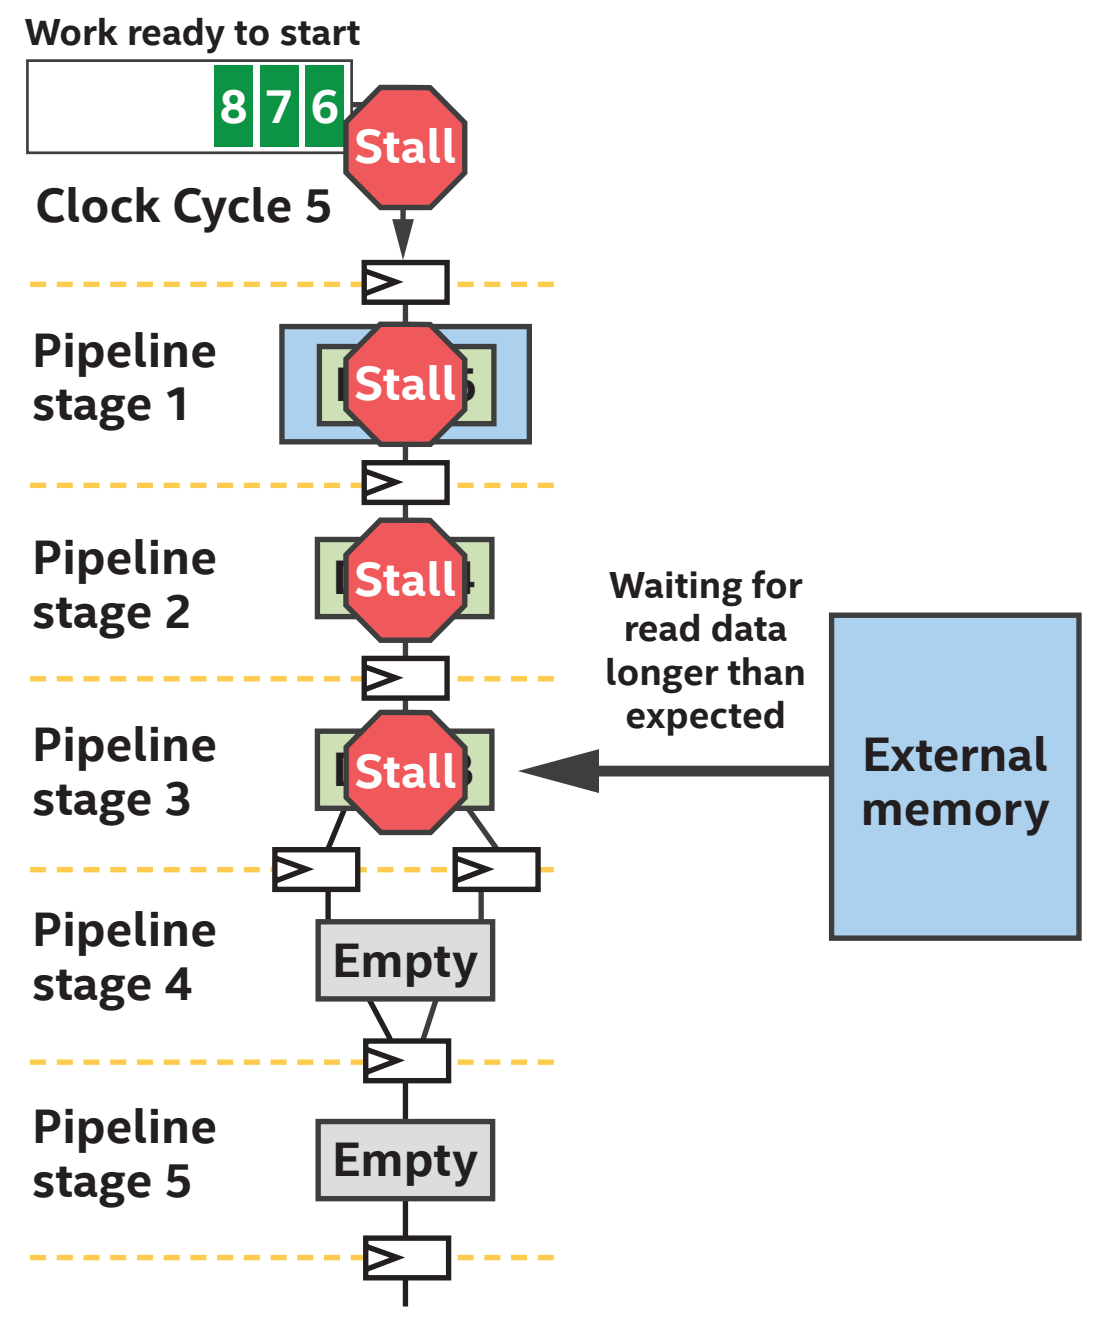
\includegraphics[width=1.0\textwidth]{content/chapter-17/images/26}
\end{center}

There are a few fronts on which memory system optimizations can be performed. As usual, the compiler reports are our primary guide to what the compiler has implemented for us and what might be worth tweaking or improving. We list a few optimization topics here to highlight some of the degrees of freedom available to us. Optimization is typically available both through explicit controls and by modifying code to allow the compiler to infer the structures that we intend. The compiler static reports and vendor documentation are key parts of memory system optimization, sometimes combined with profiling tools during hardware executions to capture actual memory behavior for validation or for the final stages of tuning.\par

\begin{enumerate}
	\item Static coalescing: The compiler will combine memory accesses into a smaller number of wider accesses, where it can. This reduces the complexity of a memory system in terms of numbers of load or store units in the pipeline, ports on the memory system, the size and complexity of arbitration networks, and other memory system details. In general, we want to enable static coalescing wherever possible, which we can confirm through the compiler reports. Simplifying addressing logic in a kernel can sometimes be enough for the compiler to perform more aggressive static coalescing, so always check in the reports that the compiler has inferred what we expect!
	\item Memory access style: The compiler creates load or store units for memory accesses, and these are tailored to both the memory technology being accessed (e.g., on-chip vs. DDR vs. HBM) and the access pattern inferred from the source code (e.g., streaming, dynamically coalesced/widened, or likely to benefit from a cache of a specific size). The compiler reports tell us what the compiler has 	inferred and allow us to modify or add controls to our code, where relevant, to improve performance.
	\item Memory system structure: Memory systems (both on- and off-chip) can have banked structures and numerous optimizations implemented by the compiler. There are many controls and mode modifications that can be used to control these structures and to tune specific aspects of the spatial 	implementation.
\end{enumerate}
















